\section{Un protocole d'échantillonnage aléatoire adaptatif}

% \begin{frame}{Communication}{Propagation des modifications}

%   Préserver la \textbf{cohérence à terme} des documents requière que tous les
%   identifiants générés par la structure de séquences soient intégrés par tous
%   les éditeurs.
  
%   \vspace{0.5cm}
  
%   Les éditeurs collaboratifs nécessitent un moyen de \textbf{communiquer} les
%   changements effectués sur le document à tous les éditeurs impliqués dans
%   l'édition.
  
%   \vspace{0.5cm}

%   \large
%   \begin{itemize}
%   \item [$\Rightarrow$] \textbf{Dissémination d'information}
%   \end{itemize}
%   \vspace{0.5cm}
% \end{frame}


% \begin{frame}{Communication}{Diffusion épidémique}
%   En \textbf{décentralisé}, la diffusion épidémique de messages constitue une
%   manière efficace de disséminer l'information. Les messages parviennent à tous
%   les pairs sans que ceux-ci ne connaissent tous les membres du réseau.

%   \vspace{0.5cm}

%   % Fonctionnement : chaque pair possède une vue partielle du réseau.
%   % \begin{enumerate}
%   % \uncover<2->{\item un pair souhaitant diffuser un message l'envoie à sa vue partielle;}
%   % \uncover<3->{\item chaque pair recevant un tel message le diffuse à sa vue partielle;}
%   % \uncover<4->{\item condition d'arrêt : le message a déjà été reçu auparavant.}
%   % \end{enumerate}

% %  \begin{minipage}{0.43\textwidth}
%     \begin{center}
%       \begin{tikzpicture}[scale=1]

\newcommand\X{40pt}
\newcommand\Y{-15pt}

\draw[->] (0*\X, 0*\Y) -- (-5+1*\X,-3*\Y);
\draw[->](0*\X, 0*\Y) -- (-5+1*\X,-0*\Y);
\draw[->] (0*\X, 0*\Y) -- (-5+1*\X, 3*\Y);

% \only<2>\draw[->, very thick] (0*\X, 0*\Y) -- (-5+1*\X,-3*\Y);
% \only<2>\draw[->, very thick](0*\X, 0*\Y) -- (-5+1*\X,-0*\Y);
% \only<2>\draw[->, very thick] (0*\X, 0*\Y) -- (-5+1*\X, 3*\Y);


\draw[->] (1*\X, 3*\Y) -- (-5+2*\X, 4*\Y);
\draw[->] (1*\X, 3*\Y) -- (-5+2*\X, 3*\Y);
\draw[->] (1*\X, 3*\Y) -- (-5+2*\X, 2*\Y);

\draw[->] (1*\X, 0*\Y) -- (-5+2*\X, 1*\Y);
\draw[->] (1*\X, 0*\Y) -- (-5+2*\X, 0*\Y);
\draw[->] (1*\X, 0*\Y) -- (-5+2*\X,-1*\Y);

\draw[->] (1*\X,-3*\Y) -- (-5+2*\X,-2*\Y);
\draw[->] (1*\X,-3*\Y) -- (-5+2*\X,-3*\Y);
\draw[->] (1*\X,-3*\Y) -- (-5+2*\X,-4*\Y);

% \only<3>\draw[->, very thick] (1*\X, 3*\Y) -- (-5+2*\X, 4*\Y);
% \only<3>\draw[->, very thick] (1*\X, 3*\Y) -- (-5+2*\X, 3*\Y);
% \only<3>\draw[->, very thick] (1*\X, 3*\Y) -- (-5+2*\X, 2*\Y);

% \only<3>\draw[->, very thick] (1*\X, 0*\Y) -- (-5+2*\X, 1*\Y);
% \only<3>\draw[->, very thick] (1*\X, 0*\Y) -- (-5+2*\X, 0*\Y);
% \only<3>\draw[->, very thick] (1*\X, 0*\Y) -- (-5+2*\X,-1*\Y);

% \only<3>\draw[->, very thick] (1*\X,-3*\Y) -- (-5+2*\X,-2*\Y);
% \only<3>\draw[->, very thick] (1*\X,-3*\Y) -- (-5+2*\X,-3*\Y);
% \only<3>\draw[->, very thick] (1*\X,-3*\Y) -- (-5+2*\X,-4*\Y);


%\draw[<-, very thick, color=white] (5+1*\X, 5-3*\Y)to[out=90,in=140](-5+2*\X, 5-4*\Y);
%\draw[<-] (5+1*\X, 5-3*\Y)to[out=90,in=140](-5+2*\X, 5-4*\Y);
% \only<4>\draw[<-, very thick] (5+1*\X, 5-3*\Y)to[out=90,in=140](-5+2*\X, 5-4*\Y);
% \only<4>{\draw[fill=white, very thick] ( 2*\X, -4*\Y) node{$e_a$} +(-5pt,-5pt) rectangle +(5pt,5pt);}

%% ea --- ec
\draw[->](2*\X, -4*\Y) -- (3*\X, 5-4*\Y);
\draw[->](2*\X, -4*\Y) -- (3*\X, -5-4*\Y);
\draw[->](2*\X, -4*\Y) -- (3*\X, -0-4*\Y);
%\draw[->](2*\X, -4*\Y) -- (3*\X,  5-4*\Y);

\draw[->](2*\X, -3*\Y) -- (3*\X, -5-3*\Y);
\draw[->](2*\X, -3*\Y) -- (3*\X, -0-3*\Y);
\draw[->](2*\X, -3*\Y) -- (3*\X,  5-3*\Y);

\draw[->](2*\X, -2*\Y) -- (3*\X, -5-2*\Y);
\draw[->](2*\X, -2*\Y) -- (3*\X, -0-2*\Y);
\draw[->](2*\X, -2*\Y) -- (3*\X,  5-2*\Y);

%% ed --- ef
\draw[->](2*\X, -1*\Y) -- (3*\X, -5-1*\Y);
\draw[->](2*\X, -1*\Y) -- (3*\X, -0-1*\Y);
\draw[->](2*\X, -1*\Y) -- (3*\X,  5-1*\Y);

\draw[->](2*\X, -0*\Y) -- (3*\X, -5-0*\Y);
\draw[->](2*\X, -0*\Y) -- (3*\X, -0-0*\Y);
\draw[->](2*\X, -0*\Y) -- (3*\X,  5-0*\Y);

\draw[->](2*\X, 1*\Y) -- (3*\X, -5+1*\Y);
\draw[->](2*\X, 1*\Y) -- (3*\X, -0+1*\Y);
\draw[->](2*\X, 1*\Y) -- (3*\X,  5+1*\Y);

%% eg --- ei
\draw[->](2*\X, 2*\Y) -- (3*\X, -5+2*\Y);
\draw[->](2*\X, 2*\Y) -- (3*\X, -0+2*\Y);
\draw[->](2*\X, 2*\Y) -- (3*\X,  5+2*\Y);

\draw[->](2*\X, 3*\Y) -- (3*\X, -5+3*\Y);
\draw[->](2*\X, 3*\Y) -- (3*\X, -0+3*\Y);
\draw[->](2*\X, 3*\Y) -- (3*\X,  5+3*\Y);

\draw[->](2*\X, 4*\Y) -- (3*\X, -5+4*\Y);
\draw[->](2*\X, 4*\Y) -- (3*\X, -0+4*\Y);
\draw[->](2*\X, 4*\Y) -- (3*\X,  5+4*\Y);


%% ea --- ec
% \only<4>\draw[->, very thick](2*\X, -4*\Y) -- (3*\X, -5-4*\Y);
% \only<4>\draw[->, very thick](2*\X, -4*\Y) -- (3*\X, -0-4*\Y);
% %\only<4>\draw[->, very thick](2*\X, -4*\Y) -- (3*\X,  5-4*\Y);

% \only<4>\draw[->, very thick](2*\X, -3*\Y) -- (3*\X, -5-3*\Y);
% \only<4>\draw[->, very thick](2*\X, -3*\Y) -- (3*\X, -0-3*\Y);
% \only<4>\draw[->, very thick](2*\X, -3*\Y) -- (3*\X,  5-3*\Y);

% \only<4>\draw[->, very thick](2*\X, -2*\Y) -- (3*\X, -5-2*\Y);
% \only<4>\draw[->, very thick](2*\X, -2*\Y) -- (3*\X, -0-2*\Y);
% \only<4>\draw[->, very thick](2*\X, -2*\Y) -- (3*\X,  5-2*\Y);

% %% ed --- ef
% \only<4>\draw[->, very thick](2*\X, -1*\Y) -- (3*\X, -5-1*\Y);
% \only<4>\draw[->, very thick](2*\X, -1*\Y) -- (3*\X, -0-1*\Y);
% \only<4>\draw[->, very thick](2*\X, -1*\Y) -- (3*\X,  5-1*\Y);

% \only<4>\draw[->, very thick](2*\X, -0*\Y) -- (3*\X, -5-0*\Y);
% \only<4>\draw[->, very thick](2*\X, -0*\Y) -- (3*\X, -0-0*\Y);
% \only<4>\draw[->, very thick](2*\X, -0*\Y) -- (3*\X,  5-0*\Y);

% \only<4>\draw[->, very thick](2*\X, 1*\Y) -- (3*\X, -5+1*\Y);
% \only<4>\draw[->, very thick](2*\X, 1*\Y) -- (3*\X, -0+1*\Y);
% \only<4>\draw[->, very thick](2*\X, 1*\Y) -- (3*\X,  5+1*\Y);

% %% eg --- ei
% \only<4>\draw[->, very thick](2*\X, 2*\Y) -- (3*\X, -5+2*\Y);
% \only<4>\draw[->, very thick](2*\X, 2*\Y) -- (3*\X, -0+2*\Y);
% \only<4>\draw[->, very thick](2*\X, 2*\Y) -- (3*\X,  5+2*\Y);

% \only<4>\draw[->, very thick](2*\X, 3*\Y) -- (3*\X, -5+3*\Y);
% \only<4>\draw[->, very thick](2*\X, 3*\Y) -- (3*\X, -0+3*\Y);
% \only<4>\draw[->, very thick](2*\X, 3*\Y) -- (3*\X,  5+3*\Y);

% \only<4>\draw[->, very thick](2*\X, 4*\Y) -- (3*\X, -5+4*\Y);
% \only<4>\draw[->, very thick](2*\X, 4*\Y) -- (3*\X, -0+4*\Y);
% \only<4>\draw[->, very thick](2*\X, 4*\Y) -- (3*\X,  5+4*\Y);



\draw[fill=white] ( 0*\X, 0*\Y) node{$e$} +(-5pt,-5pt) rectangle +(5pt,5pt);
% \only<2>{\draw[fill=white, very thick] ( 0*\X, 0*\Y) node{$e$} +(-5pt,-5pt) rectangle +(5pt,5pt);}

\draw[fill=white] ( 1*\X,-3*\Y) node{$e_1$} +(-5pt,-5pt) rectangle +(5pt,5pt);
\draw[fill=white] ( 1*\X, 0*\Y) node{$e_2$} +(-5pt,-5pt) rectangle +(5pt,5pt);
\draw[fill=white] ( 1*\X, 3*\Y) node{$e_3$} +(-5pt,-5pt) rectangle +(5pt,5pt);

% \only<3>{\draw[fill=white, very thick] ( 1*\X,-3*\Y) node{$e_1$} +(-5pt,-5pt) rectangle +(5pt,5pt);}
% \only<3>{\draw[fill=white, very thick] ( 1*\X, 0*\Y) node{$e_2$} +(-5pt,-5pt) rectangle +(5pt,5pt);}
% \only<3>{\draw[fill=white, very thick] ( 1*\X, 3*\Y) node{$e_3$} +(-5pt,-5pt) rectangle +(5pt,5pt);}


\draw[fill=white] ( 2*\X, -4*\Y) node{$e_a$} +(-5pt,-5pt) rectangle +(5pt,5pt);
\draw[fill=white] ( 2*\X, -3*\Y) node{$e_b$} +(-5pt,-5pt) rectangle +(5pt,5pt);
\draw[fill=white] ( 2*\X, -2*\Y) node{$e_c$} +(-5pt,-5pt) rectangle +(5pt,5pt);

\draw[fill=white] ( 2*\X, -1*\Y) node{$e_d$} +(-5pt,-5pt) rectangle +(5pt,5pt);
\draw[fill=white] ( 2*\X,  0*\Y) node{$e_e$} +(-5pt,-5pt) rectangle +(5pt,5pt);
\draw[fill=white] ( 2*\X,  1*\Y) node{$e_f$} +(-5pt,-5pt) rectangle +(5pt,5pt);

\draw[fill=white] ( 2*\X,  2*\Y) node{$e_g$} +(-5pt,-5pt) rectangle +(5pt,5pt);
\draw[fill=white] ( 2*\X,  3*\Y) node{$e_h$} +(-5pt,-5pt) rectangle +(5pt,5pt);
\draw[fill=white] ( 2*\X,  4*\Y) node{$e_i$} +(-5pt,-5pt) rectangle +(5pt,5pt);

% \only<4>{\draw[fill=white, very thick] ( 2*\X, -4*\Y) node{$e_a$} +(-5pt,-5pt) rectangle +(5pt,5pt);}
% \only<4>{\draw[fill=white, very thick] ( 2*\X, -3*\Y) node{$e_b$} +(-5pt,-5pt) rectangle +(5pt,5pt);}
% \only<4>{\draw[fill=white, very thick] ( 2*\X, -2*\Y) node{$e_c$} +(-5pt,-5pt) rectangle +(5pt,5pt);}

% \only<4>{\draw[fill=white, very thick] ( 2*\X, -1*\Y) node{$e_d$} +(-5pt,-5pt) rectangle +(5pt,5pt);}
% \only<4>{\draw[fill=white, very thick] ( 2*\X,  0*\Y) node{$e_e$} +(-5pt,-5pt) rectangle +(5pt,5pt);}
% \only<4>{\draw[fill=white, very thick] ( 2*\X,  1*\Y) node{$e_f$} +(-5pt,-5pt) rectangle +(5pt,5pt);}

% \only<4>{\draw[fill=white, very thick] ( 2*\X,  2*\Y) node{$e_g$} +(-5pt,-5pt) rectangle +(5pt,5pt);}
% \only<4>{\draw[fill=white, very thick] ( 2*\X,  3*\Y) node{$e_h$} +(-5pt,-5pt) rectangle +(5pt,5pt);}
% \only<4>{\draw[fill=white, very thick] ( 2*\X,  4*\Y) node{$e_i$} +(-5pt,-5pt) rectangle +(5pt,5pt);}



\end{tikzpicture}
%     \end{center}
% %  \end{minipage}
% %  \hfill
% %  \begin{minipage}{0.55\textwidth}

%     \vspace{0.5cm}
%     \large
%     \begin{itemize}
%       %\uncover<5->{
%     \item [$\Rightarrow$] \textbf{Comment configurer la taille
%           des vues partielles et les peupler ?}
%       \begin{itemize}
%       \item [$\rightarrow$] Protocole d'échantillonnage de pairs
%       \end{itemize}
%       % }
%     \end{itemize}
% %  \end{minipage}

% \end{frame}

\begin{frame}{Communication}{Contexte Web}


  N'importe quel outil informatique ayant accès à l'internet peut rejoindre une
  session d'édition.
  \begin{itemize}
  \item [$\rightarrow$] capacité hétérogènes et parfois limitées.    
  \end{itemize}

  \vspace{0.5cm}
  
  Facilite l'accès à un grand nombre d'utilisateurs.
  \begin{itemize}
  \item [$\rightarrow$] nombre fluctuant d'utilisateurs au cours du temps
  \end{itemize}


  
  \vspace{0.5cm}

  La diffusion d'informations et d'idées dans le Web est extrêmement rapide. 
  \begin{itemize}
  \item [$\rightarrow$] expose au pic soudains de popularité.
  \end{itemize}

%  capacités hétérogènes et parfois limitées des outils de
%    navigation;
%  \item le contexte Web expose aux \textbf{pics soudains de popularité.}

 
  \vspace{0.5cm}
  \large
  \begin{itemize}
  \item [$\Rightarrow$] \textbf{Le réseau doit pouvoir supporter la haute
      dynamicité induite par le Web.}
  \end{itemize}

\end{frame}



% \begin{frame}{Communication}{Contexte Web}
  
%   \begin{minipage}{0.69\textwidth}
%     Le contexte \textbf{Web} pousse à la \textbf{centralisation :}
%     \begin{itemize}
%     \item problèmes de \textbf{confidentialité}, \textbf{censure}, etc.
%     \uncover<2->{\item problèmes de passage à l'échelle, notamment en \textbf{nombre de
%         collaborateurs};}
%     \uncover<3->{\item problèmes de \textbf{résilience} aux pannes.}
%     \end{itemize}
%   \end{minipage}
%   \hfill
%   \begin{minipage}{0.3\textwidth}
%     
\includegraphics[width=0.7\textwidth]{img/www.png}
%   \end{minipage}

%   \vspace{0.75cm}
  

%   \begin{minipage}{0.32\textwidth}
%     \begin{center}
%       \begin{tikzpicture}
%         \node[visible on=<1-3>]
%         {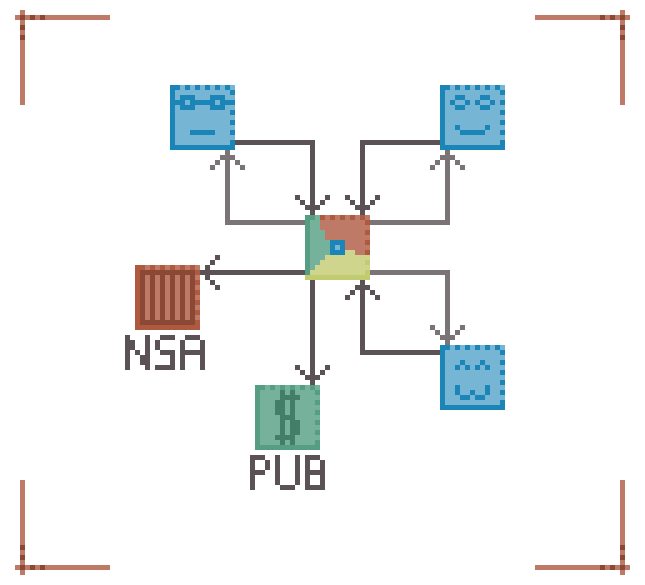
\includegraphics[width=0.95\textwidth]{img/centralizedethicproblems.png}};
%       \end{tikzpicture}
%     \end{center}
%   \end{minipage}
%   \begin{minipage}{0.32\textwidth}
%     \begin{center}
%       \begin{tikzpicture}
%         \node[visible on=<2-3>]
%         {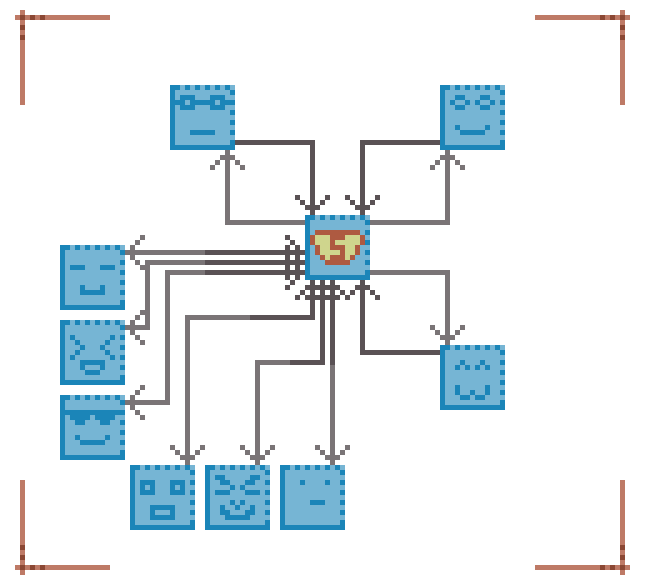
\includegraphics[width=0.95\textwidth]{img/centralizedcpuproblems.png}};
%       \end{tikzpicture}
%     \end{center}
%   \end{minipage}
%   \begin{minipage}{0.32\textwidth}
%     \begin{center}
%       \begin{tikzpicture}
%         \node[visible on=<3-3>]
%         {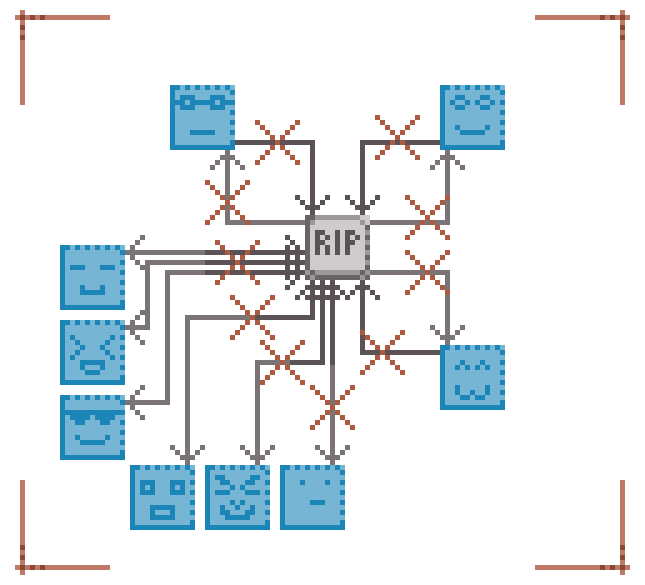
\includegraphics[width=0.95\textwidth]{img/centralizedscalabilityproblems.png}};
%       \end{tikzpicture}        
%     \end{center}
%   \end{minipage}
% \end{frame}


\begin{frame}{Communication}{Un seul moyen de communiquer : WebRTC}


  \begin{minipage}{0.67\textwidth}
    Seulement depuis récemment, et grâce à WebRTC, les navigateurs Web ne sont
    plus seulement des clients mais aussi des \textbf{serveurs}.
  \end{minipage}
  \hfill
  \begin{minipage}{0.3\textwidth}
    \begin{center}
    
\includegraphics[width=0.6\textwidth]{img/webrtc.png}
    \end{center}
  \end{minipage}
  
  % \vspace{0.5cm}
  \begin{itemize}
  \item \textbf{ni adresses ni routes};
  \item les connexions sont \textbf{coûteuses} et sujettes aux
    \textbf{défaillances};
%  \item \textbf{capacités hétérogènes et parfois limitées} des outils de
%    navigation;
%  \item le contexte Web expose aux \textbf{pics soudains de popularité.}
  \end{itemize}
  
  \vspace{0.5cm}

  % \begin{minipage}{0.6\textwidth}
  %   Pour créer un réseau : 
  %   \begin{itemize}
  %     \uncover<2->{\item Un \textbf{serveur sert de médiateur} à la connexion initiale;
  %     \begin{itemize}
  %     \item [$\rightarrow$] Au moins 1 aller-retour de messages 
  %     \end{itemize}}
  %     \uncover<3->{\item Les pairs \textbf{deviennent des médiateurs} du réseau;}
  %     \uncover<4>{\item Réseau de trois membres avec connexions directes.}
  %   \end{itemize}
  % \end{minipage}
  % \begin{minipage}{0.3\textwidth}
  %   \begin{center}
  %     
\begin{tikzpicture}[scale=1.1]

\newcommand\X{40pt};
\newcommand\Y{15pt};

\draw( 1.7*\X, 0); %% spacing
\draw(-1.7*\X, 0); %% spacing

\draw[fill=white,very thick](0*\X, 0*\Y) 
node{serveur de signalement} +(-45pt,-5pt) rectangle +(45pt,5pt);

\small
\only<2>{\draw[->,dashed, very thick](-5 -1*\X, 5-2*\Y) --
node[anchor=east]{1} (-20pt,-5pt);
\draw[<-,dashed, very thick]( 5 -1*\X, 5-2*\Y) --
node[anchor=west]{4} (-10pt,-5pt);

\draw[<-,dashed, very thick](-5pt,  5-3*\Y) --
node[anchor=east]{2}(-5pt,-5pt);
\draw[->,dashed, very thick](5pt , 5-3*\Y) --
node[anchor=west]{3} (5pt,-5pt);}


\draw[fill=white]
(-1*\X,-2*\Y) node{$n_1$} +(-5pt,-5pt) rectangle +(5pt,5pt);
\draw[fill=white]
(0*\X, -3*\Y) node{$n_2$} +(-5pt,-5pt) rectangle +(5pt,5pt);
\draw[fill=white] (1*\X, -2*\Y) node{$n_3$} +(-5pt,-5pt) rectangle +(5pt,5pt);


\small
\only<3>{
\draw[<->, very thick](5-1*\X,-2*\Y)--
node[anchor=south]{1$\rightarrow$}
node[anchor=north]{$\leftarrow$4}(-5pt,-3*\Y);
\draw[<->, very thick](5pt,-3*\Y)--
node[anchor=south]{2$\rightarrow$}
node[anchor=north]{$\leftarrow$3}(-5+1*\X,-2*\Y);
}


\only<4>{
\draw[<->](5-1*\X,-2*\Y)--(-5pt,-3*\Y);
\draw[<->](5pt,-3*\Y)--(-5+1*\X,-2*\Y);
\draw[<->, very thick](5 - 1*\X, 2.5 -2*\Y)--(-5+1*\X, 2.5 -2*\Y);
}


\end{tikzpicture}

  %   \end{center}
  % \end{minipage}
  
  
  \vspace{0.5cm}
  
  \large
  \begin{itemize}
  \item [$\Rightarrow$] \textbf{Le réseau doit supporter ce processus complexe
      d'établissement de connexion.}
  \end{itemize}
  

  
\end{frame}

% \begin{frame}{Communication}{Création de réseau}


% \end{frame}


\begin{frame}{Communication}{Définition du problème}

\begin{block}{Un protocole d'échantillonnage adaptatif}
  Soit $t$ une unité de temps arbitraire, soit $\mathcal{N}^t$ l'ensemble des
  membres non-byzantins du réseau à un instant $t$ et soit $P_i^t$ la vue
  partielle du nœud $n_i \in \mathcal{N}^t$. Un protocole d'échantillonnage
  aléatoire de pairs efficace doit assurer les propriétés suivantes :
  \begin{enumerate}
  \item Taille des vues partielles : \hfill $\forall n_i \in \mathcal{N}^t$,
    $|P_i^t| \approx \mathcal{O}(\ln |\mathcal{N}^t|)$
  \item Établissement de connexion : \hfill $\mathcal{O}(1)$
%  \item \TODO{Convergence}
  \end{enumerate}
\end{block}

\begin{itemize}
\item [$\rightarrow$] Les vues partielles reflètent les besoins du réseau;
\item [$\rightarrow$] Limiter le nombre de sauts pour établir une connexion.
\end{itemize}


\end{frame}


% \begin{frame}{Communication}{État de l'art}

% %\vspace{0.5cm}
  
%   \begin{itemize}
%   \item Vues de taille fixe configurées a priori 
%   \end{itemize}
  
%   \begin{exampleblock}{Dans un cours en ligne ouvert et massif \ldots}
%     \ldots un cours peut commencer avec énormément d'étudiants; rapidement
%     perdre en popularité à mesure que l'intérêt des étudiants décline; voir sa
%     population croître lorsque les examens finaux arrivent.
%   \end{exampleblock}
  
%   \vspace{0.5cm}

% %  \begin{minipage}{0.37\textwidth}
%   \begin{itemize}
%   \item Protocole peu adapté au type de connexion WebRTC
%   \end{itemize}
%   % L'établissement de connexion nécessite au moins 1 aller-retour de message.
% %\end{minipage}
% %\begin{minipage}{0.61\textwidth}
%   \begin{center}
%     \begin{tikzpicture}[scale=1.]

\newcommand\X{40pt}
\newcommand\Y{-40pt}

  \draw (-\X, 0); %% align texts

  \small
  \draw (0pt,5pt)node[align=left,anchor=south]{$1_{initie}$\\
    $3_{ach\grave{e}ve}$};
  \draw (2*\X, 5pt)node[anchor=south east]{$2_{accepte}^{Cyclon}$};
  \draw(4*\X,5pt)node[anchor=south]{$2_{accepte}^{Scamp}$};
  \draw (3.5*\X, 0.5*\Y)node{\DARKBLUE{\ldots}};

  \draw[dashed](2*\X,-5pt)--(2*\X,-5+1*\Y);
  \draw[dashed](2*\X, 5pt)--(2*\X, 20pt);

  \normalsize
  \draw[fill=white, thick, draw=darkblue] (0pt, 0pt)
  node{\DARKBLUE{$n_1$}} +(-5pt,-5pt) rectangle +(5pt,5pt);
  \draw[fill=white] (1*\X,\Y) node{$n_2$} +(-5pt,-5pt) rectangle +(5pt,5pt);
  \draw[fill=white] (2*\X, 0pt) node{$n_3$} +(-5pt,-5pt) rectangle +(5pt,5pt);
  \draw[fill=white] (3*\X,\Y) node{$n_4$} +(-5pt,-5pt) rectangle +(5pt,5pt);
  \draw[fill=white, thick, draw=darkblue] (4*\X, 0pt) node{\DARKBLUE{$n_k$}}
  +(-5pt,-5pt) rectangle +(5pt,5pt);


  \draw[->] ( 0pt,-5pt) to[out=-85,in=175] (-5+1*\X,\Y);
  \draw[->, densely dashed] (1*\X, 5+\Y) to[out=95,in=-5] ( 5pt, 0pt);
  \draw     ( 5+1*\X, \Y) to[out=5,in=-95] (2*\X,-5pt);
  \draw[densely dashed] ( -5+2*\X, 0pt) to[out=185,in=85] (1*\X, 5+\Y);
  \draw[->] (2*\X, -5pt) to[out=-85,in=175] (-5+3*\X, \Y);
  \draw[->, densely dashed] (3*\X, 5+\Y) to[out=95,in=-5] (5+2*\X,0pt);
  \draw[->] (5+3*\X, \Y) to[out=5pt,in=-95] (4*\X,-5pt);
  \draw[densely dashed] (-5+4*\X, 0pt) to[out=185,in=85] (3*\X, 5+\Y);
%%  \draw[->, densely dashed] (-70pt, 0pt) -- (-30pt, 0pt); %% u1 -> u4
%%  \draw[->, densely dashed] (-5pt, 30pt) -- (-70pt, 5pt); %% u3 -> u1
%%  \draw[->, densely dashed] (30pt, -5pt) to[out=-85,in=-95](-70pt,-5pt);%%u5 u1

  \small 
  \begin{scope}[shift={(4.5*\X,0pt)}]
    \draw[->](0pt, -12pt)--(10pt, -12pt) node[anchor=west]{Aller};
    \draw[->, densely dashed](0pt, -19pt)--(10pt, -19pt)
    node[anchor=west]{Retour};    
  \end{scope}
  
\end{tikzpicture}
%   \end{center}
% %\end{minipage}





% \end{frame}



\begin{frame}{Communication}{\SPRAY}

  \SPRAY est un protocole d'échantillonnage aléatoire de pairs
  \textbf{adaptatif} supportant le processus complexe d'établissement de
  connexions WebRTC.

  \vspace{0.5cm}

  % Chaque pair réagit à des événements et agit périodiquement. Le système
  % converge rapidement vers une topologie possédant des propriétés similaires à
  % celles des graphes aléatoires.

  Le réseau est \textbf{dynamique} : à n'importe quel moment, un pair peut
  rejoindre ou quitter le réseau. \\
  
  \vspace{0.5cm}

  Invariant : nombre de connexions $\approx |\mathcal{N}| \log |\mathcal{N}|$,
  sans connaissance globale, i.e., $|\mathcal{N}|$ n'est connu de personne.

  \vspace{1cm}

  \begin{minipage}{0.32\textwidth}
    \begin{center}
      \begin{tikzpicture}{scale=1}

  \newcommand\X{65pt};
  \newcommand\Y{15pt};


  \draw[->] (5+0*\X, 0*\Y) -- node[anchor=north]{\small{rejoint}} (-27+1*\X, 0*\Y);

  \draw[fill=white, very thick, draw=darkblue]
  (0*\X, 0*\Y) node{\DARKBLUE{$n$}} +(-5pt,-5pt) rectangle +(5pt,5pt);
  

  \draw[fill=white, dashed]
  (1*\X, 0*\Y) node{réseau $|\mathcal{N}|$} +(-27pt,-25pt) rectangle +(27pt,25pt);

 
\end{tikzpicture}
    \end{center}
  \end{minipage}
  \begin{minipage}{0.32\textwidth}
    \begin{center}
      \begin{tikzpicture}{scale=1}

  \newcommand\X{65pt};
  \newcommand\Y{15pt};


%  \draw[->] (0*\X, 0*\Y) -- node{rejoint} (-27+1*\X, 0*\Y);


  \draw[fill=white, dashed]
  (0*\X, 0*\Y) +(-27pt,-25pt) rectangle +(27pt,25pt);

  \draw[fill=white, very thick, draw=darkblue]
  (0*\X, 0*\Y) node{\DARKBLUE{$n$}} +(-5pt,-5pt) rectangle +(5pt,5pt);
  
  \draw[->] (  2+0*\X, -20+0*\Y ) to[out=15,in=-15] (2+0*\X, 20+0*\Y);
  \draw[<-] ( -2+0*\X, -20+0*\Y ) to[out=165,in=-165] (-2+0*\X, 20+0*\Y);

 
\end{tikzpicture}\\
    \end{center}
  \end{minipage}
  \begin{minipage}{0.32\textwidth}
    \begin{center}
      \begin{tikzpicture}{scale=1}

  \newcommand\X{65pt};
  \newcommand\Y{15pt};


  \draw[->] (27+0*\X, 0*\Y) -- node[anchor=north]{\small{quitte}} (-5+1*\X, 0*\Y);

  \draw[fill=white, very thick, draw=darkblue]
  (1*\X, 0*\Y) node{\DARKBLUE{$n$}} +(-5pt,-5pt) rectangle +(5pt,5pt);
  

  \draw[fill=white, dashed]
  (0*\X, 0*\Y) node{réseau $|\mathcal{N}|$} +(-27pt,-25pt) rectangle +(27pt,25pt);

 
\end{tikzpicture}
    \end{center}
  \end{minipage}

  \vspace{0.15cm}

  \begin{minipage}{0.32\textwidth}
    \begin{center}
      \small Ajoute $1+\log |\mathcal{N}|$ connexions
    \end{center}
  \end{minipage}
  \begin{minipage}{0.32\textwidth}
    \begin{center}
%      \small Ajoute $1+\log |\mathcal{N}|$ connexions
    \end{center}
  \end{minipage}
  \begin{minipage}{0.32\textwidth}
    \begin{center}
      \small Retire $1+\log |\mathcal{N}|$ connexions
    \end{center}
  \end{minipage}



  % Cycle de vie d'un pair : 
  % \begin{enumerate}
  % \item \textbf{Rejoindre} le réseau;
  % \item \textbf{Rester} dans le réseau;
  % \item \textbf{Quitter} le réseau.
  % \end{enumerate}

  % \large
  % \begin{itemize}
  % \item [$\Rightarrow$] \textbf{Le nombre de connexions établies doit rester cohérent.}
  % \end{itemize}
\end{frame}


\begin{frame}{Communication}{Rejoindre le réseau}

  L'entrée d'un nouveau pair s'accompagne de $1+ \log {|\mathcal{N}|}$
  connexions.

  \vspace{0.5cm}
  
  \begin{itemize}
  \item \textbf{1 :} Le pair entrant se connecte à son contact;
  \item $\pmb{\log |\mathcal{N}|}$: On suppose que le protocole répond au
    problème et chaque pair possède une taille de vue partielle
    $\approx \log |\mathcal{N}|$.
  \end{itemize}

  \vspace{1cm}

  \begin{minipage}{0.32\textwidth}
    \begin{center}
      
\begin{tikzpicture}[scale=1.1]

  \newcommand\X{35pt};
  \newcommand\Y{15pt};

%  \draw(-0.75*\X, 0pt); %% positioning
%  \draw( 2.75*\X, 0pt); %% positioning

  \scriptsize
  \draw[->,dashed,very thick, color=darkblue](5+0*\X, 0*\Y) -- 
  node[anchor=south]{(a)}(-5+ 2*\X, 0*\Y);
  \draw[->] (-5+2*\X, 5pt) -- (5+\X, \Y);
  \draw[->] (-5+2*\X, 5pt) --  (5+\X, 2*\Y);
  \draw[->] (-5+2*\X, -5pt) -- (5+\X, -\Y);
  \draw[->] (-5+2*\X, -5pt) -- (5+\X, -2*\Y);

  \normalsize
  \draw[fill=white, very thick, draw=darkblue]
  (0*\X, 0*\Y) node{\DARKBLUE{$n_1$}} +(-5pt,-5pt) rectangle +(5pt,5pt);
  \draw[fill=white, very thick]
  (2*\X, 0*\Y) node{$n_2$} +(-5pt,-5pt) rectangle +(5pt,5pt);

  \draw[fill=white](1*\X,2*\Y) node{$n_6$} +(-5pt,-5pt) rectangle +(5pt,5pt);
  \draw[fill=white](1*\X,1*\Y) node{$n_5$} +(-5pt,-5pt) rectangle +(5pt,5pt);
  \draw[fill=white](1*\X,-1*\Y) node{$n_4$} +(-5pt,-5pt) rectangle +(5pt,5pt);
  \draw[fill=white](1*\X,-2*\Y) node{$n_3$} +(-5pt,-5pt) rectangle +(5pt,5pt);
  
\end{tikzpicture}
    \end{center}
  \end{minipage}
  \begin{minipage}{0.32\textwidth}
    \begin{center}
      
\begin{tikzpicture}[scale=1.1]

  \newcommand\X{35pt};
  \newcommand\Y{15pt};

%  \draw(-0.75*\X, 0pt); %% positioning
%  \draw( 2.75*\X, 0pt); %% positioning

  \scriptsize
  \draw[->](5+0*\X, 0*\Y) -- (-5+ 2*\X, 0*\Y);
  \draw[->, very thick, color=darkblue] (-5+2*\X, 5pt) -- (5+\X, \Y);
  \draw[->, very thick, color=darkblue] (-5+2*\X, 5pt) --
  node[anchor=south west]{(b)} (5+\X, 2*\Y);
  \draw[->, very thick, color=darkblue] (-5+2*\X, -5pt) -- (5+\X, -\Y);
  \draw[->, very thick, color=darkblue] (-5+2*\X, -5pt) --
  node[anchor=north west]{(b)}(5+\X, -2*\Y);

  \normalsize
  \draw[fill=white]
  (0*\X, 0*\Y) node{$n_1$} +(-5pt,-5pt) rectangle +(5pt,5pt);
  \draw[fill=white, very thick, draw=darkblue]
  (2*\X, 0*\Y) node{\DARKBLUE{$n_2$}} +(-5pt,-5pt) rectangle +(5pt,5pt);

  \draw[fill=white, very thick]
  (1*\X,2*\Y) node{$n_6$} +(-5pt,-5pt) rectangle +(5pt,5pt);
  \draw[fill=white, very thick]
  (1*\X,1*\Y) node{$n_5$} +(-5pt,-5pt) rectangle +(5pt,5pt);
  \draw[fill=white, very thick]
  (1*\X,-1*\Y) node{$n_4$} +(-5pt,-5pt) rectangle +(5pt,5pt);
  \draw[fill=white, very thick]
  (1*\X,-2*\Y) node{$n_3$} +(-5pt,-5pt) rectangle +(5pt,5pt);

\end{tikzpicture}
    \end{center}
  \end{minipage}
  \begin{minipage}{0.32\textwidth}
    \begin{center}
      
\begin{tikzpicture}[scale=1.1]

  \newcommand\X{35pt};
  \newcommand\Y{15pt};

%  \draw(-0.75*\X, 0pt); %% positioning
%  \draw( 2.75*\X, 0pt); %% positioning

  \scriptsize
  \draw[->](5+0*\X, 0*\Y) -- (-5+ 2*\X, 0*\Y);
  \draw[->] (-5+2*\X, 5pt) -- (5+\X, \Y);
  \draw[->] (-5+2*\X, 5pt) -- (5+\X, 2*\Y);
  \draw[->] (-5+2*\X, -5pt) -- (5+\X, -\Y);
  \draw[->] (-5+2*\X, -5pt) -- (5+\X, -2*\Y);

  \draw[->,dashed, very thick, color=darkblue](-5+\X, 2*\Y) --
  node[anchor=south east]{(c)} ( 5pt,5pt);
  \draw[->,dashed, very thick, color=darkblue](-5+\X, 1*\Y) -- ( 5pt,5pt);
  \draw[->,dashed, very thick, color=darkblue](-5+\X, -1*\Y) -- ( 5pt,-5pt);
  \draw[->,dashed, very thick, color=darkblue](-5+\X, -2*\Y) --
  node[anchor=north east]{(c)}( 5pt,-5pt);

  \normalsize
  \draw[fill=white, very thick]
  (0*\X, 0*\Y) node{$n_1$} +(-5pt,-5pt) rectangle +(5pt,5pt);
  \draw[fill=white]
  (2*\X, 0*\Y) node{$n_2$} +(-5pt,-5pt) rectangle +(5pt,5pt);

  \draw[fill=white, very thick, draw=darkblue]
  (1*\X,2*\Y) node{\DARKBLUE{$n_6$}} +(-5pt,-5pt) rectangle +(5pt,5pt);
  \draw[fill=white, very thick, draw=darkblue]
  (1*\X,1*\Y) node{\DARKBLUE{$n_5$}} +(-5pt,-5pt) rectangle +(5pt,5pt);
  \draw[fill=white, very thick, draw=darkblue]
  (1*\X,-1*\Y) node{\DARKBLUE{$n_4$}} +(-5pt,-5pt) rectangle +(5pt,5pt);
  \draw[fill=white, very thick, draw=darkblue]
  (1*\X,-2*\Y) node{\DARKBLUE{$n_3$}} +(-5pt,-5pt) rectangle +(5pt,5pt);
 

\end{tikzpicture}
    \end{center}
  \end{minipage}



  % \begin{itemize}
  % \item [$\rightarrow$] $|\mathcal{N}|$ pairs implique
  %   $|\mathcal{N}|\ln |\mathcal{N}|$ connexions.
  % \end{itemize}


%  \vspace{0.5cm}

  % \begin{minipage}{0.6\textwidth}
  %   \begin{enumerate}[(a)]
  %   \item Le nouvel arrivant se connecte à un contact ($1$ connexion);
  %   \uncover<2->{\item Le contact dissémine la nouvelle arrivée aux membres de sa vue;}
  %   \uncover<3->{\item Chacun de ces voisins établit une connexion
  %     ($\approx \ln |\mathcal{N}|$ connexions).}
  %   \end{enumerate}
  % \end{minipage}
  % \hfill
  % \begin{minipage}{0.35\textwidth}
  %   \begin{center}
  %     
\begin{tikzpicture}[scale=1.2]

  \newcommand\X{35pt};
  \newcommand\Y{15pt};

%  \draw(-0.75*\X, 0pt); %% positioning
%  \draw( 2.75*\X, 0pt); %% positioning

\only<1>{
  \draw[fill=white, very thick, hide on=1]
  (1*\X,2*\Y) node{$n_6$} +(-5pt,-5pt) rectangle +(5pt,5pt);
  \draw[fill=white, very thick, hide on=1]
  (1*\X,-2*\Y) node{$n_3$} +(-5pt,-5pt) rectangle +(5pt,5pt);
  

  \scriptsize
  \draw[->,dashed,very thick, color=darkblue](5+0*\X, 0*\Y) -- 
  node[anchor=south]{(a)}(-5+ 2*\X, 0*\Y);
  \draw[->] (-5+2*\X, 5pt) -- (5+\X, \Y);
  \draw[->] (-5+2*\X, 5pt) --  (5+\X, 2*\Y);
  \draw[->] (-5+2*\X, -5pt) -- (5+\X, -\Y);
  \draw[->] (-5+2*\X, -5pt) -- (5+\X, -2*\Y);

  \normalsize
  \draw[fill=white, very thick, draw=darkblue]
  (0*\X, 0*\Y) node{\DARKBLUE{$n_1$}} +(-5pt,-5pt) rectangle +(5pt,5pt);
  \draw[fill=white, very thick]
  (2*\X, 0*\Y) node{$n_2$} +(-5pt,-5pt) rectangle +(5pt,5pt);

  \draw[fill=white](1*\X,2*\Y) node{$n_6$} +(-5pt,-5pt) rectangle +(5pt,5pt);
  \draw[fill=white](1*\X,1*\Y) node{$n_5$} +(-5pt,-5pt) rectangle +(5pt,5pt);
  \draw[fill=white](1*\X,-1*\Y) node{$n_4$} +(-5pt,-5pt) rectangle +(5pt,5pt);
  \draw[fill=white](1*\X,-2*\Y) node{$n_3$} +(-5pt,-5pt) rectangle +(5pt,5pt);

}

\only<2>{
  \scriptsize
  \draw[->](5+0*\X, 0*\Y) -- (-5+ 2*\X, 0*\Y);
  \draw[->, very thick, color=darkblue] (-5+2*\X, 5pt) -- (5+\X, \Y);
  \draw[->, very thick, color=darkblue] (-5+2*\X, 5pt) --
  node[anchor=south west]{(b)} (5+\X, 2*\Y);
  \draw[->, very thick, color=darkblue] (-5+2*\X, -5pt) -- (5+\X, -\Y);
  \draw[->, very thick, color=darkblue] (-5+2*\X, -5pt) --
  node[anchor=north west]{(b)}(5+\X, -2*\Y);

  \normalsize
  \draw[fill=white]
  (0*\X, 0*\Y) node{$n_1$} +(-5pt,-5pt) rectangle +(5pt,5pt);
  \draw[fill=white, very thick, draw=darkblue]
  (2*\X, 0*\Y) node{\DARKBLUE{$n_2$}} +(-5pt,-5pt) rectangle +(5pt,5pt);

  \draw[fill=white, very thick]
  (1*\X,2*\Y) node{$n_6$} +(-5pt,-5pt) rectangle +(5pt,5pt);
  \draw[fill=white, very thick]
  (1*\X,1*\Y) node{$n_5$} +(-5pt,-5pt) rectangle +(5pt,5pt);
  \draw[fill=white, very thick]
  (1*\X,-1*\Y) node{$n_4$} +(-5pt,-5pt) rectangle +(5pt,5pt);
  \draw[fill=white, very thick]
  (1*\X,-2*\Y) node{$n_3$} +(-5pt,-5pt) rectangle +(5pt,5pt);
}

\only<3->{

  \scriptsize
  \draw[->](5+0*\X, 0*\Y) -- (-5+ 2*\X, 0*\Y);
  \draw[->] (-5+2*\X, 5pt) -- (5+\X, \Y);
  \draw[->] (-5+2*\X, 5pt) -- (5+\X, 2*\Y);
  \draw[->] (-5+2*\X, -5pt) -- (5+\X, -\Y);
  \draw[->] (-5+2*\X, -5pt) -- (5+\X, -2*\Y);

  \draw[->,dashed, very thick, color=darkblue](-5+\X, 2*\Y) --
  node[anchor=south east]{(c)} ( 5pt,5pt);
  \draw[->,dashed, very thick, color=darkblue](-5+\X, 1*\Y) -- ( 5pt,5pt);
  \draw[->,dashed, very thick, color=darkblue](-5+\X, -1*\Y) -- ( 5pt,-5pt);
  \draw[->,dashed, very thick, color=darkblue](-5+\X, -2*\Y) --
  node[anchor=north east]{(c)}( 5pt,-5pt);

  \normalsize
  \draw[fill=white, very thick]
  (0*\X, 0*\Y) node{$n_1$} +(-5pt,-5pt) rectangle +(5pt,5pt);
  \draw[fill=white]
  (2*\X, 0*\Y) node{$n_2$} +(-5pt,-5pt) rectangle +(5pt,5pt);

  \draw[fill=white, very thick, draw=darkblue]
  (1*\X,2*\Y) node{\DARKBLUE{$n_6$}} +(-5pt,-5pt) rectangle +(5pt,5pt);
  \draw[fill=white, very thick, draw=darkblue]
  (1*\X,1*\Y) node{\DARKBLUE{$n_5$}} +(-5pt,-5pt) rectangle +(5pt,5pt);
  \draw[fill=white, very thick, draw=darkblue]
  (1*\X,-1*\Y) node{\DARKBLUE{$n_4$}} +(-5pt,-5pt) rectangle +(5pt,5pt);
  \draw[fill=white, very thick, draw=darkblue]
  (1*\X,-2*\Y) node{\DARKBLUE{$n_3$}} +(-5pt,-5pt) rectangle +(5pt,5pt);
}


\end{tikzpicture}
  %   \end{center}
  % \end{minipage}
  
  \vspace{1cm}
  
  \large
  \begin{itemize}
  \item [$\Rightarrow$] \textbf{Les vues partielles sont déséquilibrées}
  \end{itemize}

\end{frame}

\begin{frame}{Communication}{Échanges périodiques}
 
  Le nombre de connexions reste \textbf{constant}.
 
  \vspace{0.5cm}

  Les deux pairs impliqués dans l'échange périodique donne la \textbf{moitié} de
  leur vue partielle. Les pairs sont choisis \textbf{aléatoirement}.
  \begin{itemize}
  \item [$\rightarrow$] La taille des vues converge vers la \textbf{moyenne} des
    deux.
  \end{itemize}
  

  \vspace{0.5cm}\hspace{-1cm}
  \begin{minipage}{0.32\textwidth}
    \begin{center}
      
\begin{tikzpicture}[scale=1]

  \newcommand\X{35pt};
  \newcommand\Y{15pt};

  \draw[->](5+0*\X, 0*\Y) -- (-5+ 2*\X, 0*\Y); %% 1 -> 2
  \draw[->] (-5+2*\X, 5pt) -- (5+\X, \Y);
  \draw[->](2*\X,5pt) -- (5+1*\X, 2*\Y); %% 2 -> 6
  \draw[->] (-5+2*\X, -5pt) -- (5+\X, -\Y);
  \draw[->] (-5+2*\X, -5pt) -- (5+\X, -2*\Y);

  \draw[->,very thick, color=darkblue](-5+\X,2*\Y) -- (0pt,5pt); %% 6 -> 1

  \draw[->](-5+\X, 1*\Y) -- ( 5pt,5pt);
  \draw[->](-5+\X, -1*\Y) -- ( 5pt,-5pt);
  \draw[->](-5+\X, -2*\Y) -- ( 5pt,-5pt);

  \draw[->](-5+\X, 5+2*\Y)to[out=120,in=30](0pt,5+2*\Y); %% 6 -> 7
  \draw[->](-5+\X, 5+2*\Y)to[out=120,in=30](-5-\Y ,5+2*\Y); %% 6 -> 8
  \draw[->](-5+\X, 5+2*\Y)to[out=120,in=30](-10-2*\Y,5+2*\Y); %% 6 -> 9

  \normalsize
  \draw[fill=white, very thick]
  (0*\X, 0*\Y) node{$n_1$} +(-5pt,-5pt) rectangle +(5pt,5pt);
  \draw[fill=white](2*\X, 0*\Y) node{$n_2$} +(-5pt,-5pt) rectangle +(5pt,5pt);

  \draw[fill=white,very thick, draw=darkblue]
  (1*\X,2*\Y) node{\DARKBLUE{$n_6$}} +(-5pt,-5pt) rectangle +(5pt,5pt);
  \draw[fill=white](1*\X,1*\Y) node{$n_5$} +(-5pt,-5pt) rectangle +(5pt,5pt);
  \draw[fill=white](1*\X,-1*\Y) node{$n_4$} +(-5pt,-5pt) rectangle +(5pt,5pt);
  \draw[fill=white](1*\X,-2*\Y) node{$n_3$} +(-5pt,-5pt) rectangle +(5pt,5pt);

  \draw[fill=white]( 0*\X,2*\Y)
  node{$n_7$} +(-5pt,-5pt) rectangle +(5pt,5pt);
  \draw[fill=white](-5+-\Y,2*\Y)node{$n_8$} +(-5pt,-5pt) rectangle +(5pt,5pt);
  \draw[fill=white, draw=darkblue](-10+-2*\Y,2*\Y)
  node{\DARKBLUE{$n_9$}} +(-5pt,-5pt) rectangle +(5pt,5pt);
  

\end{tikzpicture}
    \end{center}
  \end{minipage}
  \hspace{0.35cm}
  \begin{minipage}{0.32\textwidth}
    \begin{center}
      
\begin{tikzpicture}[scale=1]

  \newcommand\X{35pt};
  \newcommand\Y{15pt};

  \draw[->](5+0*\X, 0*\Y) -- (-5+ 2*\X, 0*\Y); %% 1 -> 2
  \draw[->] (-5+2*\X, 5pt) -- (5+\X, \Y);
  \draw[->](2*\X,5pt) -- (5+1*\X, 2*\Y); %% 2 -> 6
  \draw[->] (-5+2*\X, -5pt) -- (5+\X, -\Y);
  \draw[->] (-5+2*\X, -5pt) -- (5+\X, -2*\Y);

  \draw[->,dashed, very thick, color=darkblue](0pt,5pt)--(-5+\X, 2*\Y); %% 1 -> 6

  \draw[->](-5+\X, 1*\Y) -- ( 5pt,5pt);
  \draw[->](-5+\X, -1*\Y) -- ( 5pt,-5pt);
  \draw[->](-5+\X, -2*\Y) -- ( 5pt,-5pt);

  \draw[->](-5+\X, 5+2*\Y)to[out=120,in=30](0pt,5+2*\Y); %% 6 -> 7
  \draw[->](-5+\X, 5+2*\Y)to[out=120,in=30](-5-\Y ,5+2*\Y); %% 6 -> 8
  
  \draw[->,dashed, very thick, color=darkblue](-5pt,5pt)--(-10-2*\Y,-5+2*\Y); %% 1 -> 9

  \normalsize
  \draw[fill=white, very thick]
  (0*\X, 0*\Y) node{$n_1$} +(-5pt,-5pt) rectangle +(5pt,5pt);
  \draw[fill=white, draw=darkblue](2*\X, 0*\Y)
  node{\DARKBLUE{$n_2$}} +(-5pt,-5pt) rectangle +(5pt,5pt);

  \draw[fill=white,very thick]
  (1*\X,2*\Y) node{$n_6$} +(-5pt,-5pt) rectangle +(5pt,5pt);
  \draw[fill=white](1*\X,1*\Y) node{$n_5$} +(-5pt,-5pt) rectangle +(5pt,5pt);
  \draw[fill=white](1*\X,-1*\Y) node{$n_4$} +(-5pt,-5pt) rectangle +(5pt,5pt);
  \draw[fill=white](1*\X,-2*\Y) node{$n_3$} +(-5pt,-5pt) rectangle +(5pt,5pt);

  \draw[fill=white]( 0*\X,2*\Y)
  node{$n_7$} +(-5pt,-5pt) rectangle +(5pt,5pt);
  \draw[fill=white](-5+-\Y,2*\Y)node{$n_8$} +(-5pt,-5pt) rectangle +(5pt,5pt);
  \draw[fill=white](-10+-2*\Y,2*\Y) node{$n_9$} +(-5pt,-5pt) rectangle +(5pt,5pt);
  

\end{tikzpicture}
    \end{center}
  \end{minipage}
  \hspace{0.35cm}
  \begin{minipage}{0.32\textwidth}
    \begin{center}
      
\begin{tikzpicture}[scale=1]

  \newcommand\X{35pt};
  \newcommand\Y{15pt};

  \draw[->] (-5+2*\X, 5pt) -- (5+\X, \Y);
  \draw[->,dashed, very thick, color=darkblue]
  (5+\X, 2*\Y)to[out=-20,in=110](2*\X, 5pt); %% 6 -> 2
  \draw[->](2*\X,5pt)to[out=160,in=-70](5+1*\X, 2*\Y); %% 2 -> 6
  \draw[->] (-5+2*\X, -5pt) -- (5+\X, -\Y);
  \draw[->] (-5+2*\X, -5pt) -- (5+\X, -2*\Y);

  \draw[->](0pt,5pt)--(-5+\X, 2*\Y); %% 1 -> 6

  \draw[->](-5+\X, 1*\Y) -- ( 5pt,5pt);
  \draw[->](-5+\X, -1*\Y) -- ( 5pt,-5pt);
  \draw[->](-5+\X, -2*\Y) -- ( 5pt,-5pt);

  \draw[->](-5+\X, 5+2*\Y)to[out=120,in=30](0pt,5+2*\Y); %% 6 -> 7
  \draw[->](-5+\X, 5+2*\Y)to[out=120,in=30](-5-\Y ,5+2*\Y); %% 6 -> 8
  
  \draw[->](-5pt,5pt)--(-10-2*\Y,-5+2*\Y); %% 1 -> 9

  \normalsize
  \draw[fill=white]
  (0*\X, 0*\Y) node{$n_1$} +(-5pt,-5pt) rectangle +(5pt,5pt);
  \draw[fill=white](2*\X, 0*\Y) node{$n_2$} +(-5pt,-5pt) rectangle +(5pt,5pt);

  \draw[fill=white,very thick]
  (1*\X,2*\Y) node{$n_6$} +(-5pt,-5pt) rectangle +(5pt,5pt);
  \draw[fill=white](1*\X,1*\Y) node{$n_5$} +(-5pt,-5pt) rectangle +(5pt,5pt);
  \draw[fill=white](1*\X,-1*\Y) node{$n_4$} +(-5pt,-5pt) rectangle +(5pt,5pt);
  \draw[fill=white](1*\X,-2*\Y) node{$n_3$} +(-5pt,-5pt) rectangle +(5pt,5pt);

  \draw[fill=white]( 0*\X,2*\Y)
  node{$n_7$} +(-5pt,-5pt) rectangle +(5pt,5pt);
  \draw[fill=white](-5+-\Y,2*\Y)node{$n_8$} +(-5pt,-5pt) rectangle +(5pt,5pt);
  \draw[fill=white](-10+-2*\Y,2*\Y) node{$n_9$} +(-5pt,-5pt) rectangle +(5pt,5pt);
  

\end{tikzpicture}
    \end{center}
  \end{minipage}



  % \begin{minipage}{0.6\textwidth}
  %   \begin{enumerate}[(a)]
  %   \item Initiation du mélange périodique. Le pair devient médiateur entre
  %     $\lceil P \div 2 \rceil - 1$ voisins aléatoires et le pair choisi pour le
  %     mélange. 
  %   \uncover<2->{\item En réponse, le pair choisi devient médiateur entre
  %     $\lceil P\div 2 \rceil$ voisins et le pair initiateur;}
  %   \uncover<3->{\item Le pair initiateur reçoit la réponse et établit ses 
  %     connexions grâce au pair choisi.}
  %   \end{enumerate}
  % \end{minipage}
  % \begin{minipage}{0.37\textwidth}
  %   \begin{center}
  %     
\begin{tikzpicture}[scale=1.1]

  \newcommand\X{35pt};
  \newcommand\Y{15pt};

  \draw[->, hide on=1-](-5+\X, 5+2*\Y)to[out=120,in=30](-10-2*\Y,5+2*\Y); %% 6 -> 9
\only<1>{
  \draw[->](5+0*\X, 0*\Y) -- (-5+ 2*\X, 0*\Y); %% 1 -> 2
  \draw[->] (-5+2*\X, 5pt) -- (5+\X, \Y);
  \draw[->](2*\X,5pt) -- (5+1*\X, 2*\Y); %% 2 -> 6
  \draw[->] (-5+2*\X, -5pt) -- (5+\X, -\Y);
  \draw[->] (-5+2*\X, -5pt) -- (5+\X, -2*\Y);

  \draw[->,very thick, color=darkblue](-5+\X,2*\Y) -- (0pt,5pt); %% 6 -> 1

  \draw[->](-5+\X, 1*\Y) -- ( 5pt,5pt);
  \draw[->](-5+\X, -1*\Y) -- ( 5pt,-5pt);
  \draw[->](-5+\X, -2*\Y) -- ( 5pt,-5pt);

  \draw[->](-5+\X, 5+2*\Y)to[out=120,in=30](0pt,5+2*\Y); %% 6 -> 7
  \draw[->](-5+\X, 5+2*\Y)to[out=120,in=30](-5-\Y ,5+2*\Y); %% 6 -> 8
  \draw[->](-5+\X, 5+2*\Y)to[out=120,in=30](-10-2*\Y,5+2*\Y); %% 6 -> 9

  \normalsize
  \draw[fill=white, very thick]
  (0*\X, 0*\Y) node{$n_1$} +(-5pt,-5pt) rectangle +(5pt,5pt);
  \draw[fill=white](2*\X, 0*\Y) node{$n_2$} +(-5pt,-5pt) rectangle +(5pt,5pt);

  \draw[fill=white,very thick, draw=darkblue]
  (1*\X,2*\Y) node{\DARKBLUE{$n_6$}} +(-5pt,-5pt) rectangle +(5pt,5pt);
  \draw[fill=white](1*\X,1*\Y) node{$n_5$} +(-5pt,-5pt) rectangle +(5pt,5pt);
  \draw[fill=white](1*\X,-1*\Y) node{$n_4$} +(-5pt,-5pt) rectangle +(5pt,5pt);
  \draw[fill=white](1*\X,-2*\Y) node{$n_3$} +(-5pt,-5pt) rectangle +(5pt,5pt);

  \draw[fill=white]( 0*\X,2*\Y)
  node{$n_7$} +(-5pt,-5pt) rectangle +(5pt,5pt);
  \draw[fill=white](-5+-\Y,2*\Y)node{$n_8$} +(-5pt,-5pt) rectangle +(5pt,5pt);
  \draw[fill=white, draw=darkblue](-10+-2*\Y,2*\Y)
  node{\DARKBLUE{$n_9$}} +(-5pt,-5pt) rectangle +(5pt,5pt);
}

\only<2>{
  \draw[->](5+0*\X, 0*\Y) -- (-5+ 2*\X, 0*\Y); %% 1 -> 2
  \draw[->] (-5+2*\X, 5pt) -- (5+\X, \Y);
  \draw[->](2*\X,5pt) -- (5+1*\X, 2*\Y); %% 2 -> 6
  \draw[->] (-5+2*\X, -5pt) -- (5+\X, -\Y);
  \draw[->] (-5+2*\X, -5pt) -- (5+\X, -2*\Y);

  \draw[->,dashed, very thick, color=darkblue](0pt,5pt)--(-5+\X, 2*\Y); %% 1 -> 6

  \draw[->](-5+\X, 1*\Y) -- ( 5pt,5pt);
  \draw[->](-5+\X, -1*\Y) -- ( 5pt,-5pt);
  \draw[->](-5+\X, -2*\Y) -- ( 5pt,-5pt);

  \draw[->](-5+\X, 5+2*\Y)to[out=120,in=30](0pt,5+2*\Y); %% 6 -> 7
  \draw[->](-5+\X, 5+2*\Y)to[out=120,in=30](-5-\Y ,5+2*\Y); %% 6 -> 8
  
  \draw[->,dashed, very thick, color=darkblue](-5pt,5pt)--(-10-2*\Y,-5+2*\Y); %% 1 -> 9

  \normalsize
  \draw[fill=white, very thick]
  (0*\X, 0*\Y) node{$n_1$} +(-5pt,-5pt) rectangle +(5pt,5pt);
  \draw[fill=white, draw=darkblue](2*\X, 0*\Y)
  node{\DARKBLUE{$n_2$}} +(-5pt,-5pt) rectangle +(5pt,5pt);

  \draw[fill=white,very thick]
  (1*\X,2*\Y) node{$n_6$} +(-5pt,-5pt) rectangle +(5pt,5pt);
  \draw[fill=white](1*\X,1*\Y) node{$n_5$} +(-5pt,-5pt) rectangle +(5pt,5pt);
  \draw[fill=white](1*\X,-1*\Y) node{$n_4$} +(-5pt,-5pt) rectangle +(5pt,5pt);
  \draw[fill=white](1*\X,-2*\Y) node{$n_3$} +(-5pt,-5pt) rectangle +(5pt,5pt);

  \draw[fill=white]( 0*\X,2*\Y)
  node{$n_7$} +(-5pt,-5pt) rectangle +(5pt,5pt);
  \draw[fill=white](-5+-\Y,2*\Y)node{$n_8$} +(-5pt,-5pt) rectangle +(5pt,5pt);
  \draw[fill=white](-10+-2*\Y,2*\Y) node{$n_9$} +(-5pt,-5pt) rectangle +(5pt,5pt);
}


\only<3->{
  \draw[->] (-5+2*\X, 5pt) -- (5+\X, \Y);
  \draw[->,dashed, very thick, color=darkblue]
  (5+\X, 2*\Y)to[out=-20,in=110](2*\X, 5pt); %% 6 -> 2
  \draw[->](2*\X,5pt)to[out=160,in=-70](5+1*\X, 2*\Y); %% 2 -> 6
  \draw[->] (-5+2*\X, -5pt) -- (5+\X, -\Y);
  \draw[->] (-5+2*\X, -5pt) -- (5+\X, -2*\Y);

  \draw[->](0pt,5pt)--(-5+\X, 2*\Y); %% 1 -> 6

  \draw[->](-5+\X, 1*\Y) -- ( 5pt,5pt);
  \draw[->](-5+\X, -1*\Y) -- ( 5pt,-5pt);
  \draw[->](-5+\X, -2*\Y) -- ( 5pt,-5pt);

  \draw[->](-5+\X, 5+2*\Y)to[out=120,in=30](0pt,5+2*\Y); %% 6 -> 7
  \draw[->](-5+\X, 5+2*\Y)to[out=120,in=30](-5-\Y ,5+2*\Y); %% 6 -> 8
  
  \draw[->](-5pt,5pt)--(-10-2*\Y,-5+2*\Y); %% 1 -> 9

  \normalsize
  \draw[fill=white]
  (0*\X, 0*\Y) node{$n_1$} +(-5pt,-5pt) rectangle +(5pt,5pt);
  \draw[fill=white](2*\X, 0*\Y) node{$n_2$} +(-5pt,-5pt) rectangle +(5pt,5pt);

  \draw[fill=white,very thick]
  (1*\X,2*\Y) node{$n_6$} +(-5pt,-5pt) rectangle +(5pt,5pt);
  \draw[fill=white](1*\X,1*\Y) node{$n_5$} +(-5pt,-5pt) rectangle +(5pt,5pt);
  \draw[fill=white](1*\X,-1*\Y) node{$n_4$} +(-5pt,-5pt) rectangle +(5pt,5pt);
  \draw[fill=white](1*\X,-2*\Y) node{$n_3$} +(-5pt,-5pt) rectangle +(5pt,5pt);

  \draw[fill=white]( 0*\X,2*\Y)
  node{$n_7$} +(-5pt,-5pt) rectangle +(5pt,5pt);
  \draw[fill=white](-5+-\Y,2*\Y)node{$n_8$} +(-5pt,-5pt) rectangle +(5pt,5pt);
  \draw[fill=white](-10+-2*\Y,2*\Y) node{$n_9$} +(-5pt,-5pt) rectangle +(5pt,5pt);
}

\end{tikzpicture}
  %   \end{center}
  % \end{minipage}


  \vspace{0.5cm}
  \large
  \begin{itemize}
  \item [$\Rightarrow$] \textbf{Équilibre rapidement la taille des vues
      partielles;}
  \item [$\Rightarrow$] \textbf{Disperse les groupes fortement connectés.}
  \end{itemize}
  
\end{frame}

\begin{frame}{Communication}{Quitter le réseau}

  Le départ d'un pair doit engendrer la suppression de $1+\log|\mathcal{N}|$ connexions.

  \vspace{0.5cm}

  Problème : la vue sortante + la vue entrante $\approx 2\log|\mathcal{N}|$
  \begin{itemize}
  \item $\pmb{\log|\mathcal{N}|}$ : La vue partielle du pair quittant le réseau;
  \item \textbf{1} : Un parmis les $\approx \log|\mathcal{N}|$ pairs détectant
    le départ ne recrée pas de connexion.
  \end{itemize}

  \vspace{0.5cm}\hspace{-1cm}
  \begin{minipage}{0.32\textwidth}
    \begin{center}
      
\begin{tikzpicture}[scale=0.9]

  \newcommand\X{35pt};
  \newcommand\Y{15pt};

  \large
  \draw[->](-5+\X, 1*\Y) --node{$\times$} ( 5pt,5pt);
  \draw[->](-5+\X, -1*\Y) --node{$\times$} ( 5pt,-5pt);
  \draw[->](-5+\X, -2*\Y) --node{$\times$} ( 5pt,-5pt);

  \draw[->, color=darkblue](-5pt,5pt)--
  node{\DARKBLUE{$\times$}}(-10-2*\Y,-5+2*\Y); %% 1 -> 9
  \draw[->, color=darkblue](-5pt,5pt)--
  node{\DARKBLUE{$\times$}}(-5-1*\Y,-5+2*\Y); %% 1 ->8 
  \draw[->, color=darkblue](-5pt,5pt)--
  node{\DARKBLUE{$\times$}}(0pt,-5+2*\Y); %% 1 -> 7
  \draw[->, color=darkblue](-5pt,5pt)--
  node{\DARKBLUE{$\times$}}(-5+\X,-5+2*\Y); %% 1 -> 6

  \normalsize
  \draw[->](5+ 1*\X, 5+ 1*\Y)--(-5+2*\X, 2*\Y); %% 5 -> 14
  \draw[->](5+1*\X,  1*\Y)--(-5+2*\X, 1*\Y); %% 5 -> 13 
  
  \draw[->](5+\X, 5-\Y) -- (-5+2*\X,0pt); %% 4 -> 12
  \draw[->](5+\X, -\Y) -- (-5+2*\X, -\Y); %% 4 -> 11
  
  \draw[->](5+\X, -2*\Y) -- (-5+2*\X, -2*\Y);
  
  \tiny
  \draw[fill=white,very thick, draw=darkblue]
  (0*\X, 0*\Y) node{\DARKBLUE{$n_1$}} +(-5pt,-5pt) rectangle +(5pt,5pt);
  \draw[thick, color=darkblue] (-5pt,-5pt) -- (5pt,5pt);
  \draw[thick, color=darkblue] (-5pt, 5pt) -- (5pt,-5pt);
  
  \draw[fill=white]
  (1*\X,1*\Y) node{$n_5$} +(-5pt,-5pt) rectangle +(5pt,5pt);
  \draw[fill=white]
  (1*\X,-1*\Y) node{$n_4$} +(-5pt,-5pt) rectangle +(5pt,5pt);
  \draw[fill=white]
  (1*\X,-2*\Y) node{$n_3$} +(-5pt,-5pt) rectangle +(5pt,5pt);

  \draw[fill=white](\X,2*\Y) node{$n_6$} +(-5pt,-5pt) rectangle +(5pt,5pt);

  \draw[fill=white]( 0*\X,2*\Y)
  node{$n_7$} +(-5pt,-5pt) rectangle +(5pt,5pt);
  \draw[fill=white](-5+-\Y,2*\Y)node{$n_8$} +(-5pt,-5pt) rectangle +(5pt,5pt);
  \draw[fill=white](-10+-2*\Y,2*\Y) node{$n_9$} +(-5pt,-5pt) rectangle +(5pt,5pt);
  
  \draw[fill=white](2*\X,2*\Y)node{$n_{14}$} +(-5pt,-5pt) rectangle +(5pt,5pt);
  \draw[fill=white](2*\X,1*\Y)node{$n_{13}$} +(-5pt,-5pt) rectangle +(5pt,5pt);
  \draw[fill=white](2*\X,0*\Y)node{$n_{12}$} +(-5pt,-5pt) rectangle +(5pt,5pt);
  \draw[fill=white](2*\X,-1*\Y)node{$n_{11}$}+(-5pt,-5pt) rectangle +(5pt,5pt);
  \draw[fill=white](2*\X,-2*\Y)node{$n_{10}$}+(-5pt,-5pt) rectangle +(5pt,5pt);

\end{tikzpicture}
    \end{center}
  \end{minipage}
  \hspace{0.45cm}
  \begin{minipage}{0.32\textwidth}
    \begin{center}
      
\begin{tikzpicture}[scale=0.9]

  \newcommand\X{35pt};
  \newcommand\Y{15pt};

  \large
  \draw[->, very thick, color=darkblue](-5+\X, 1*\Y) --
  node{\DARKBLUE{$\times$}} ( 5pt,5pt);
  \draw[->, very thick, color=darkblue](-5+\X, -1*\Y) --
  node{\DARKBLUE{$\times$}} ( 5pt,-5pt);
  \draw[->, very thick, color=darkblue](-5+\X, -2*\Y) --
  node{\DARKBLUE{$\times$}} ( 5pt,-5pt);

  \normalsize

  \draw[->](5+ 1*\X, 5+ 1*\Y)--(-5+2*\X, 2*\Y); %% 5 -> 14
  \draw[->](  5+1*\X, 1*\Y)--(-5+2*\X, 1*\Y); %% 5 -> 13 (v)
  
  \draw[->](5+\X, 5-\Y) -- (-5+2*\X,0pt); %% 4 -> 12
  \draw[->](5+\X, -\Y) -- (-5+2*\X, -\Y); %% 4 -> 11
  
  \draw[->](5+\X, -2*\Y) -- (-5+2*\X, -2*\Y);
  
  \tiny
  \draw[fill=white]
  (0*\X, 0*\Y) node{$n_1$} +(-5pt,-5pt) rectangle +(5pt,5pt);
  \draw (-5pt,-5pt) -- (5pt,5pt);
  \draw (-5pt, 5pt) -- (5pt,-5pt);
  
  \draw[fill=white, very thick, draw=darkblue]
  (1*\X,1*\Y) node{\DARKBLUE{$n_5$}} +(-5pt,-5pt) rectangle +(5pt,5pt);
  \draw[fill=white, very thick, draw=darkblue]
  (1*\X,-1*\Y) node{\DARKBLUE{$n_4$}} +(-5pt,-5pt) rectangle +(5pt,5pt);
  \draw[fill=white, very thick, draw=darkblue]
  (1*\X,-2*\Y) node{\DARKBLUE{$n_3$}} +(-5pt,-5pt) rectangle +(5pt,5pt);

  \draw[fill=white](\X,2*\Y) node{$n_6$} +(-5pt,-5pt) rectangle +(5pt,5pt);

  \draw[fill=white]( 0*\X,2*\Y)
  node{$n_7$} +(-5pt,-5pt) rectangle +(5pt,5pt);
  \draw[fill=white](-5+-\Y,2*\Y)node{$n_8$} +(-5pt,-5pt) rectangle +(5pt,5pt);
  \draw[fill=white](-10+-2*\Y,2*\Y) node{$n_9$} +(-5pt,-5pt) rectangle +(5pt,5pt);
  
  \draw[fill=white](2*\X,2*\Y)node{$n_{14}$} +(-5pt,-5pt) rectangle +(5pt,5pt);
  \draw[fill=white](2*\X,1*\Y)node{$n_{13}$} +(-5pt,-5pt) rectangle +(5pt,5pt);
  \draw[fill=white](2*\X,0*\Y)node{$n_{12}$} +(-5pt,-5pt) rectangle +(5pt,5pt);
  \draw[fill=white](2*\X,-1*\Y)node{$n_{11}$}+(-5pt,-5pt) rectangle +(5pt,5pt);
  \draw[fill=white](2*\X,-2*\Y)node{$n_{10}$}+(-5pt,-5pt) rectangle +(5pt,5pt);

\end{tikzpicture}
    \end{center}
  \end{minipage}
  \hspace{0.45cm}
  \begin{minipage}{0.32\textwidth}
    \begin{center}
      
\begin{tikzpicture}[scale=0.9]

  \newcommand\X{35pt};
  \newcommand\Y{15pt};

  \draw[->](5+ 1*\X, 5+ 1*\Y)--(-5+2*\X, 2*\Y); %% 5 -> 14
  \draw[->](5+1*\X, 2.5+ 1*\Y)--(-5+2*\X, 2.5+ 1*\Y); %% 5 -> 13 (^)
  \draw[->,dashed, very thick, color=darkblue]
  (  5+1*\X,-2.5+1*\Y)--(-5+2*\X,-2.5+1*\Y); %% 5 -> 13 (v)
  
  \draw[->](5+\X, 5-\Y) -- (-5+2*\X,0pt); %% 4 -> 12
  \draw[->](5+\X, -\Y) -- (-5+2*\X, -\Y); %% 4 -> 11
  
  \draw[->](5+\X, 2.5-2*\Y) -- (-5+2*\X, 2.5-2*\Y);
  \draw[->,dashed, very thick, color=darkblue](5+\X, -2.5-2*\Y) -- (-5+2*\X , -2.5-2*\Y);
  
  \tiny
  \draw[fill=white]
  (0*\X, 0*\Y) node{$n_1$} +(-5pt,-5pt) rectangle +(5pt,5pt);
  \draw (-5pt,-5pt) -- (5pt,5pt);
  \draw (-5pt, 5pt) -- (5pt,-5pt);
  
  \draw[fill=white, very thick]
  (1*\X,1*\Y) node{$n_5$} +(-5pt,-5pt) rectangle +(5pt,5pt);
  \draw[fill=white, very thick]
  (1*\X,-1*\Y) node{$n_4$} +(-5pt,-5pt) rectangle +(5pt,5pt);
  \draw[fill=white, very thick]
  (1*\X,-2*\Y) node{$n_3$} +(-5pt,-5pt) rectangle +(5pt,5pt);

  \draw[fill=white](\X,2*\Y) node{$n_6$} +(-5pt,-5pt) rectangle +(5pt,5pt);

  \draw[fill=white]( 0*\X,2*\Y)
  node{$n_7$} +(-5pt,-5pt) rectangle +(5pt,5pt);
  \draw[fill=white](-5+-\Y,2*\Y)node{$n_8$} +(-5pt,-5pt) rectangle +(5pt,5pt);
  \draw[fill=white](-10+-2*\Y,2*\Y) node{$n_9$} +(-5pt,-5pt) rectangle +(5pt,5pt);
  
  \draw[fill=white](2*\X,2*\Y)node{$n_{14}$} +(-5pt,-5pt) rectangle +(5pt,5pt);
  \draw[fill=white](2*\X,1*\Y)node{$n_{13}$} +(-5pt,-5pt) rectangle +(5pt,5pt);
  \draw[fill=white](2*\X,0*\Y)node{$n_{12}$} +(-5pt,-5pt) rectangle +(5pt,5pt);
  \draw[fill=white](2*\X,-1*\Y)node{$n_{11}$}+(-5pt,-5pt) rectangle +(5pt,5pt);
  \draw[fill=white](2*\X,-2*\Y)node{$n_{10}$}+(-5pt,-5pt) rectangle +(5pt,5pt);

\end{tikzpicture}
    \end{center}
  \end{minipage}


  % \vspace{0.5cm}

  % \begin{minipage}{0.6\textwidth}
  %   \begin{enumerate}[(a)]
  %   \item Un pair quitte le réseau ou tombe en panne;
  %   \uncover<2->{\item Les pairs ayant une connexion vers lui s'aperçoivent de sa disparition;}
  %   \uncover<3->{\item Ces pairs ajoutent de manière probabiliste des doublons.}
  %   \end{enumerate}
  % \end{minipage}
  % \hfill
  % \begin{minipage}{0.37\textwidth}
  %   \begin{center}
  %     
\begin{tikzpicture}[scale=1.1]

  \newcommand\X{35pt};
  \newcommand\Y{15pt};

\draw[fill=white, very thick, draw=darkblue, hide on=1-]
(1*\X,-2*\Y) node{\DARKBLUE{$n_3$}} +(-5pt,-5pt) rectangle +(5pt,5pt);


\only<1>{
  \large
  \draw[->](-5+\X, 1*\Y) --node{$\times$} ( 5pt,5pt);
  \draw[->](-5+\X, -1*\Y) --node{$\times$} ( 5pt,-5pt);
  \draw[->](-5+\X, -2*\Y) --node{$\times$} ( 5pt,-5pt);

  \draw[->, color=darkblue](-5pt,5pt)--
  node{\DARKBLUE{$\times$}}(-10-2*\Y,-5+2*\Y); %% 1 -> 9
  \draw[->, color=darkblue](-5pt,5pt)--
  node{\DARKBLUE{$\times$}}(-5-1*\Y,-5+2*\Y); %% 1 ->8 
  \draw[->, color=darkblue](-5pt,5pt)--
  node{\DARKBLUE{$\times$}}(0pt,-5+2*\Y); %% 1 -> 7
  \draw[->, color=darkblue](-5pt,5pt)--
  node{\DARKBLUE{$\times$}}(-5+\X,-5+2*\Y); %% 1 -> 6

  \normalsize
  \draw[->](5+ 1*\X, 5+ 1*\Y)--(-5+2*\X, 2*\Y); %% 5 -> 14
  \draw[->](5+1*\X,  1*\Y)--(-5+2*\X, 1*\Y); %% 5 -> 13 
  
  \draw[->](5+\X, 5-\Y) -- (-5+2*\X,0pt); %% 4 -> 12
  \draw[->](5+\X, -\Y) -- (-5+2*\X, -\Y); %% 4 -> 11
  
  \draw[->](5+\X, -2*\Y) -- (-5+2*\X, -2*\Y);
  
  \small
  \draw[fill=white,very thick, draw=darkblue]
  (0*\X, 0*\Y) node{\DARKBLUE{$n_1$}} +(-5pt,-5pt) rectangle +(5pt,5pt);
  \draw[thick, color=darkblue] (-5pt,-5pt) -- (5pt,5pt);
  \draw[thick, color=darkblue] (-5pt, 5pt) -- (5pt,-5pt);
  
  \draw[fill=white]
  (1*\X,1*\Y) node{$n_5$} +(-5pt,-5pt) rectangle +(5pt,5pt);
  \draw[fill=white]
  (1*\X,-1*\Y) node{$n_4$} +(-5pt,-5pt) rectangle +(5pt,5pt);
  \draw[fill=white]
  (1*\X,-2*\Y) node{$n_3$} +(-5pt,-5pt) rectangle +(5pt,5pt);

  \draw[fill=white](\X,2*\Y) node{$n_6$} +(-5pt,-5pt) rectangle +(5pt,5pt);

  \draw[fill=white]( 0*\X,2*\Y)
  node{$n_7$} +(-5pt,-5pt) rectangle +(5pt,5pt);
  \draw[fill=white](-5+-\Y,2*\Y)node{$n_8$} +(-5pt,-5pt) rectangle +(5pt,5pt);
  \draw[fill=white](-10+-2*\Y,2*\Y) node{$n_9$} +(-5pt,-5pt) rectangle +(5pt,5pt);
  
  \draw[fill=white](2*\X,2*\Y)node{$n_{14}$} +(-5pt,-5pt) rectangle +(5pt,5pt);
  \draw[fill=white](2*\X,1*\Y)node{$n_{13}$} +(-5pt,-5pt) rectangle +(5pt,5pt);
  \draw[fill=white](2*\X,0*\Y)node{$n_{12}$} +(-5pt,-5pt) rectangle +(5pt,5pt);
  \draw[fill=white](2*\X,-1*\Y)node{$n_{11}$}+(-5pt,-5pt) rectangle +(5pt,5pt);
  \draw[fill=white](2*\X,-2*\Y)node{$n_{10}$}+(-5pt,-5pt) rectangle +(5pt,5pt);

}


\only<2>{

  \large
  \draw[->, very thick, color=darkblue](-5+\X, 1*\Y) --
  node{\DARKBLUE{$\times$}} ( 5pt,5pt);
  \draw[->, very thick, color=darkblue](-5+\X, -1*\Y) --
  node{\DARKBLUE{$\times$}} ( 5pt,-5pt);
  \draw[->, very thick, color=darkblue](-5+\X, -2*\Y) --
  node{\DARKBLUE{$\times$}} ( 5pt,-5pt);

  \normalsize

  \draw[->](5+ 1*\X, 5+ 1*\Y)--(-5+2*\X, 2*\Y); %% 5 -> 14
  \draw[->](  5+1*\X, 1*\Y)--(-5+2*\X, 1*\Y); %% 5 -> 13 (v)
  
  \draw[->](5+\X, 5-\Y) -- (-5+2*\X,0pt); %% 4 -> 12
  \draw[->](5+\X, -\Y) -- (-5+2*\X, -\Y); %% 4 -> 11
  
  \draw[->](5+\X, -2*\Y) -- (-5+2*\X, -2*\Y);
  
  \small
  \draw[fill=white]
  (0*\X, 0*\Y) node{$n_1$} +(-5pt,-5pt) rectangle +(5pt,5pt);
  \draw (-5pt,-5pt) -- (5pt,5pt);
  \draw (-5pt, 5pt) -- (5pt,-5pt);
  
  \draw[fill=white, very thick, draw=darkblue]
  (1*\X,1*\Y) node{\DARKBLUE{$n_5$}} +(-5pt,-5pt) rectangle +(5pt,5pt);
  \draw[fill=white, very thick, draw=darkblue]
  (1*\X,-1*\Y) node{\DARKBLUE{$n_4$}} +(-5pt,-5pt) rectangle +(5pt,5pt);
  \draw[fill=white, very thick, draw=darkblue]
  (1*\X,-2*\Y) node{\DARKBLUE{$n_3$}} +(-5pt,-5pt) rectangle +(5pt,5pt);

  \draw[fill=white](\X,2*\Y) node{$n_6$} +(-5pt,-5pt) rectangle +(5pt,5pt);

  \draw[fill=white]( 0*\X,2*\Y)
  node{$n_7$} +(-5pt,-5pt) rectangle +(5pt,5pt);
  \draw[fill=white](-5+-\Y,2*\Y)node{$n_8$} +(-5pt,-5pt) rectangle +(5pt,5pt);
  \draw[fill=white](-10+-2*\Y,2*\Y) node{$n_9$} +(-5pt,-5pt) rectangle +(5pt,5pt);
  
  \draw[fill=white](2*\X,2*\Y)node{$n_{14}$} +(-5pt,-5pt) rectangle +(5pt,5pt);
  \draw[fill=white](2*\X,1*\Y)node{$n_{13}$} +(-5pt,-5pt) rectangle +(5pt,5pt);
  \draw[fill=white](2*\X,0*\Y)node{$n_{12}$} +(-5pt,-5pt) rectangle +(5pt,5pt);
  \draw[fill=white](2*\X,-1*\Y)node{$n_{11}$}+(-5pt,-5pt) rectangle +(5pt,5pt);
  \draw[fill=white](2*\X,-2*\Y)node{$n_{10}$}+(-5pt,-5pt) rectangle +(5pt,5pt);
}

\only<3->{

  \draw[->](5+ 1*\X, 5+ 1*\Y)--(-5+2*\X, 2*\Y); %% 5 -> 14
  \draw[->](5+1*\X, 2.5+ 1*\Y)--(-5+2*\X, 2.5+ 1*\Y); %% 5 -> 13 (^)
  \draw[->,dashed, very thick, color=darkblue]
  (  5+1*\X,-2.5+1*\Y)--(-5+2*\X,-2.5+1*\Y); %% 5 -> 13 (v)
  
  \draw[->](5+\X, 5-\Y) -- (-5+2*\X,0pt); %% 4 -> 12
  \draw[->](5+\X, -\Y) -- (-5+2*\X, -\Y); %% 4 -> 11
  
  \draw[->](5+\X, 2.5-2*\Y) -- (-5+2*\X, 2.5-2*\Y);
  \draw[->,dashed, very thick, color=darkblue](5+\X, -2.5-2*\Y) -- (-5+2*\X , -2.5-2*\Y);
  
  \small
  \draw[fill=white]
  (0*\X, 0*\Y) node{$n_1$} +(-5pt,-5pt) rectangle +(5pt,5pt);
  \draw (-5pt,-5pt) -- (5pt,5pt);
  \draw (-5pt, 5pt) -- (5pt,-5pt);
  
  \draw[fill=white, very thick]
  (1*\X,1*\Y) node{$n_5$} +(-5pt,-5pt) rectangle +(5pt,5pt);
  \draw[fill=white, very thick]
  (1*\X,-1*\Y) node{$n_4$} +(-5pt,-5pt) rectangle +(5pt,5pt);
  \draw[fill=white, very thick]
  (1*\X,-2*\Y) node{$n_3$} +(-5pt,-5pt) rectangle +(5pt,5pt);

  \draw[fill=white](\X,2*\Y) node{$n_6$} +(-5pt,-5pt) rectangle +(5pt,5pt);

  \draw[fill=white]( 0*\X,2*\Y)
  node{$n_7$} +(-5pt,-5pt) rectangle +(5pt,5pt);
  \draw[fill=white](-5+-\Y,2*\Y)node{$n_8$} +(-5pt,-5pt) rectangle +(5pt,5pt);
  \draw[fill=white](-10+-2*\Y,2*\Y) node{$n_9$} +(-5pt,-5pt) rectangle +(5pt,5pt);
  
  \draw[fill=white](2*\X,2*\Y)node{$n_{14}$} +(-5pt,-5pt) rectangle +(5pt,5pt);
  \draw[fill=white](2*\X,1*\Y)node{$n_{13}$} +(-5pt,-5pt) rectangle +(5pt,5pt);
  \draw[fill=white](2*\X,0*\Y)node{$n_{12}$} +(-5pt,-5pt) rectangle +(5pt,5pt);
  \draw[fill=white](2*\X,-1*\Y)node{$n_{11}$}+(-5pt,-5pt) rectangle +(5pt,5pt);
  \draw[fill=white](2*\X,-2*\Y)node{$n_{10}$}+(-5pt,-5pt) rectangle +(5pt,5pt);

}

\end{tikzpicture}
  %   \end{center}
  % \end{minipage}

  \vspace{1cm}
  \large
  \begin{itemize}
  \item [$\Rightarrow$] \textbf{Présence de doublons assure la cohérence du
      nombre de connexions.}
  \end{itemize}
 
\end{frame}


\begin{frame}{Communication}{Expérimentations}

  Simulations \PEERSIM.

  \vspace{0.5cm}

  \begin{itemize}
  \item \CYCLON : vue partielle dont la taille est configurée \textit{a priori};
%  \item \SCAMP : vue partielle dont la taille s'ajuste au réseau;
  \item \SPRAY : vue partielles dont la taille s'ajuste au réseau et adapté au
    contexte Web.
  \end{itemize}

%\end{frame}

%\begin{frame}{Communication}{Résultats attendus}
  
  \vspace{0.5cm}


  Résultats attendus :
  \begin{itemize}
  \item Convergence rapide vers un réseau possédant des propriétés similaires à
    celles des graphes aléatoires;
  \item Les doublons sont peu nombreux et n'impactent pas significativement les
    propriétés du réseau;
  \item Les protocoles basés sur \SPRAY bénéficient de son adaptativité.
  \end{itemize}

\end{frame}


\begin{frame}{Communication}{Les vues partielles s'adaptent}
  % \hspace{-1cm}
  % \begin{minipage}{0.47\textwidth}
  %   \begin{center}
  %     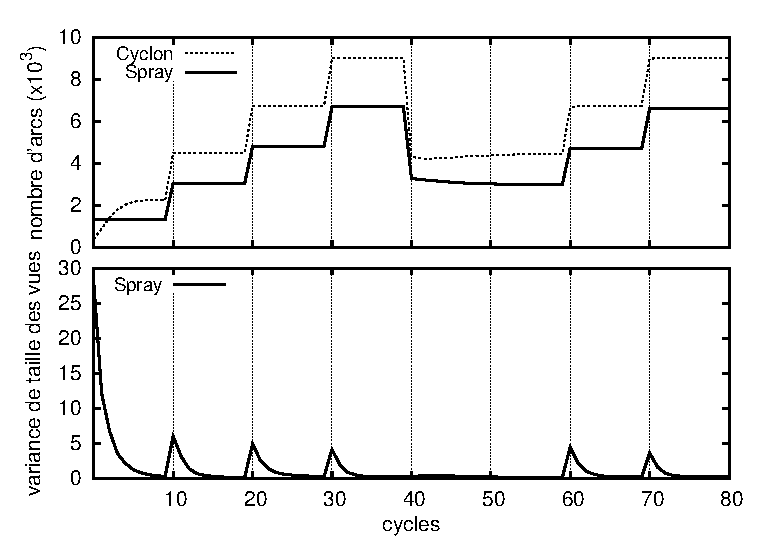
\includegraphics[width=1.23\textwidth]{img/network/churn.eps}
  %   \end{center}
  % \end{minipage}
  % \hfill
  % \begin{minipage}{0.47\textwidth}
  %     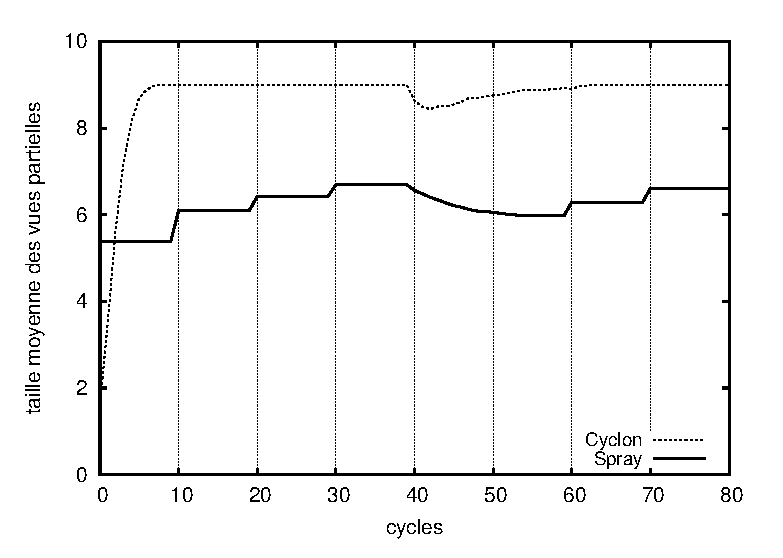
\includegraphics[width=1.23\textwidth]{img/network/avgpv.eps}
  % \end{minipage}
  \begin{center}
    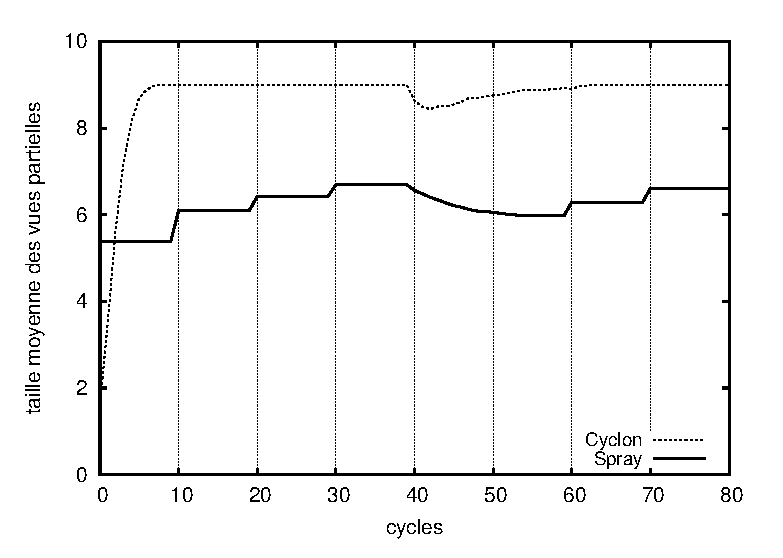
\includegraphics[width=1\textwidth]{img/network/avgpv.eps}
  \end{center}
  \begin{center}
    $250+250+250+250-500+250+250$
  \end{center}
\end{frame}



\begin{frame}{Communication}{Coefficient d'agglomération diminue rapidement}
  \hspace{-1cm}
  \begin{minipage}{0.47\textwidth}
    \begin{center}
      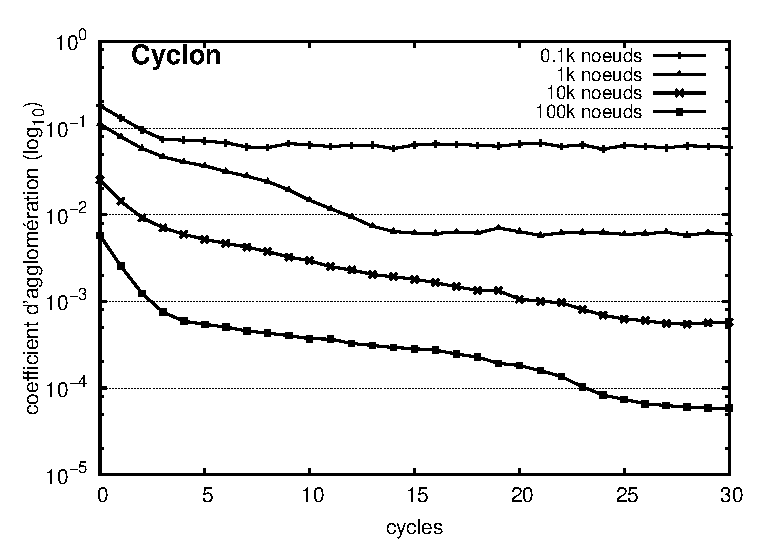
\includegraphics[width=1.23\textwidth]{img/network/cycloncluster.eps}
    \end{center}
  \end{minipage}
  \hfill
  \begin{minipage}{0.47\textwidth}
      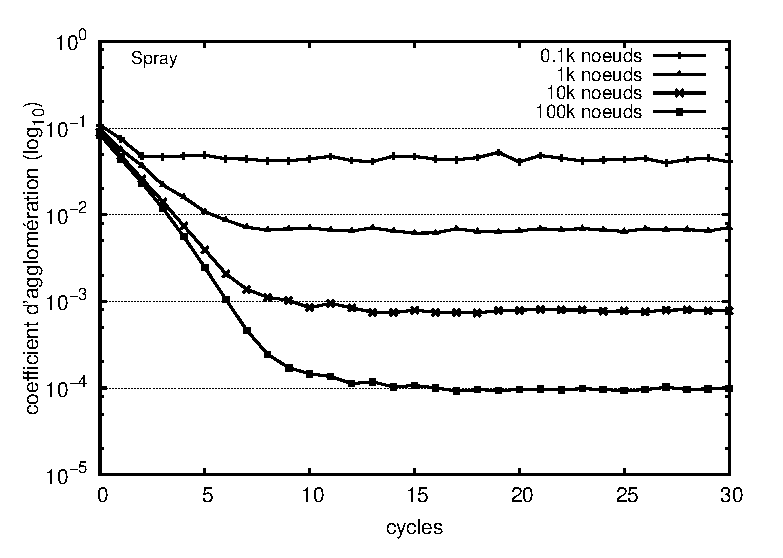
\includegraphics[width=1.23\textwidth]{img/network/spraycluster.eps}
  \end{minipage}

  \vspace{0.5cm}

  \begin{itemize}
  \item \CYCLON configuré avec
    \begin{itemize}
    \item  $\ln(1000) \approx 7$ voisins et
    \item mélange de $3$ voisins.
    \end{itemize}
  \end{itemize}

\end{frame}


\begin{frame}{Communication}{L'information se propage rapidement}
  \begin{center}
    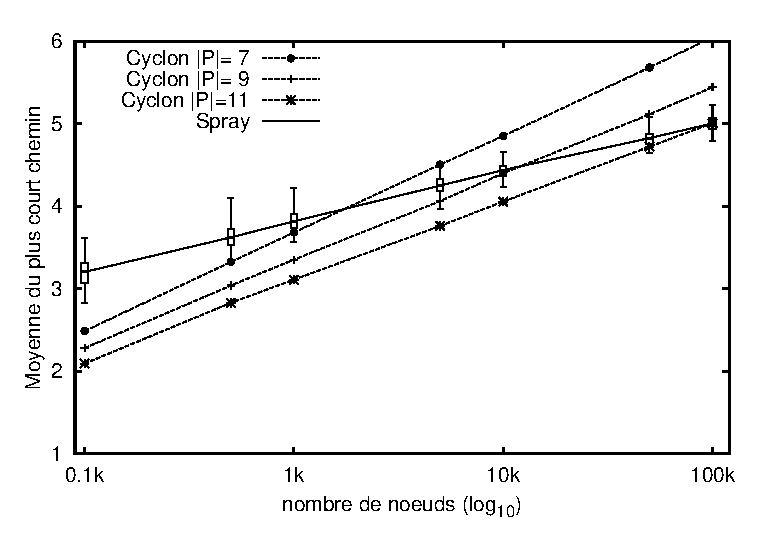
\includegraphics[width=1\textwidth]{img/network/avgpath.eps}
  \end{center}
\end{frame}

% \begin{frame}{Communication}{La charge est équilibrée}
%   \begin{center}
%     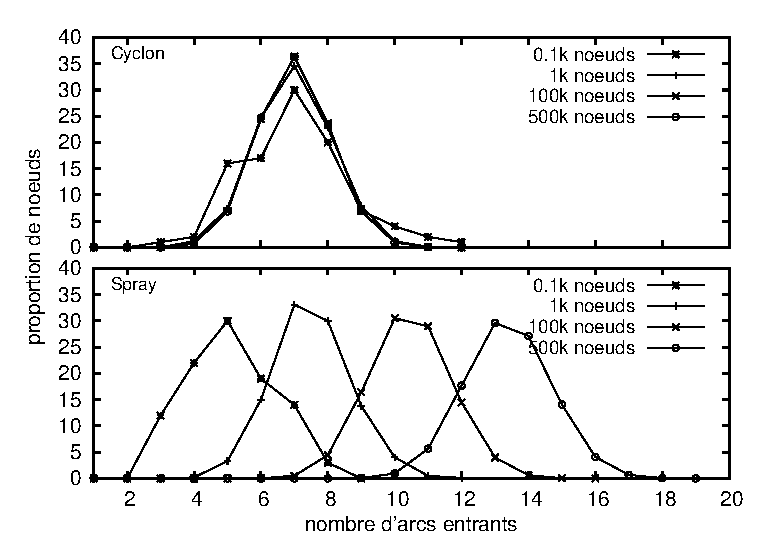
\includegraphics[width=1\textwidth]{img/network/histo.eps}
%   \end{center}
% \end{frame}


% \begin{frame}{Communication}{Robuste aux défaillances}
%   \begin{center}
%     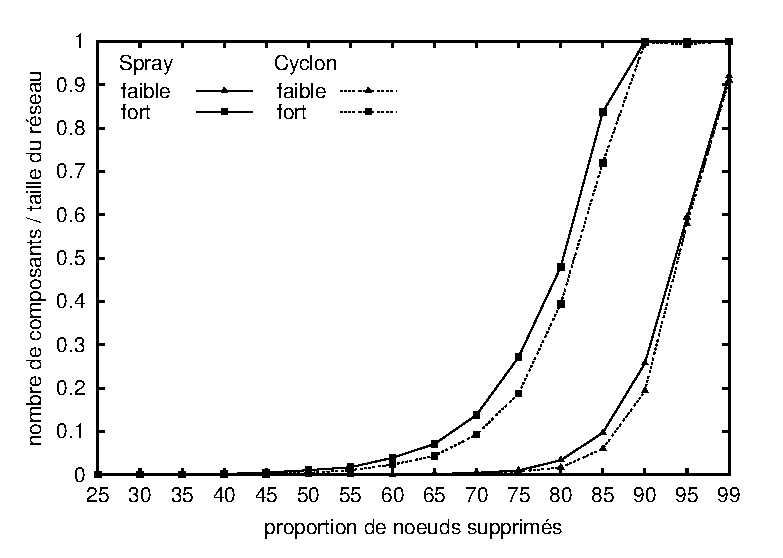
\includegraphics[width=1\textwidth]{img/network/resilience.eps}
%   \end{center}
% \end{frame}


\begin{frame}{Communication}{Faible taux de doublons}
  \begin{center}
    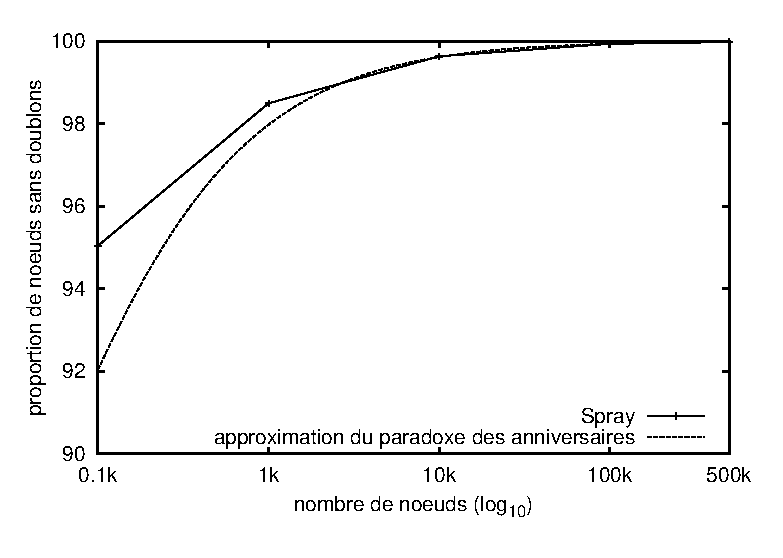
\includegraphics[width=1\textwidth]{img/network/duplicates.eps}
  \end{center}
\end{frame}


\begin{frame}{Communication}{Cas de la diffusion de messages}
  \begin{algorithm}[H]
    
\small
\algrenewcommand{\algorithmiccomment}[1]{\hskip2em$\rhd$ #1}

\newcommand{\comment}[1]{\hfill $\rhd$ #1}

\newcommand{\LINEFOR}[2]{%
  \algorithmicfor\ {#1}\ \algorithmicdo\ {#2} %
  }

\newcommand{\LINEIFTHEN}[2]{%
  \algorithmicif\ {#1}\ \algorithmicthen\ {#2} %
  }

\newcommand{\INDSTATE}[1][1]{\State\hspace{\algorithmicindent}}

\begin{algorithmic}[1]
  \Function{broadcast}{$m$} \comment{$m$: \emph{message à envoyer}}
  \State \textbf{let} $chosen \leftarrow getPeers(P,\, \DARKBLUE{fanout})$;
  \For{(\DARKBLUE{$n \in chosen$})}
  \State \textsc{sendTo}($n$, 'broadcast', $m$);
  \EndFor
  \EndFunction

  \Statex

  \Function{onBroadcast}{$m$} \comment{$m$: \emph{message reçu}}
  \If {($\DARKBLUE{\neg}$\DARKBLUE{\textsc{alreadyReceived}}$\DARKBLUE{(m)}$)}
  \State \textsc{broadcast}($m$);
  \EndIf
  \EndFunction
\end{algorithmic}

  \end{algorithm}

  \begin{itemize}
  \item \CYCLON 
    \begin{enumerate}
    \item vue partielle de 30 voisins, fanout de $\ln(100)+1\approx 6$;
    \item vue partielle de 30 voisins, fanout de  $\ln(100)+3 \approx 8$.
    \end{enumerate}
  \item \SPRAY
    \begin{enumerate}
    \item vue partielle de $6\cdot\ln|\mathcal{N}|$ voisins,
      fanout de $\ln(|\mathcal{N}|)+1$;
    \item vue partielle de $6\cdot\ln|\mathcal{N}|$ voisins,
      fanout de $\ln(|\mathcal{N}|)+3$;
    \end{enumerate}
  \end{itemize}

%  \vspace{0.5cm}

  \begin{itemize}
  \item[$\rightarrow$] \CYCLON et \SPRAY sont équivalent à 100 pairs
  \end{itemize}
\end{frame}

\begin{frame}{Communication}{Le taux d'erreur reste constant}
  \begin{center}
    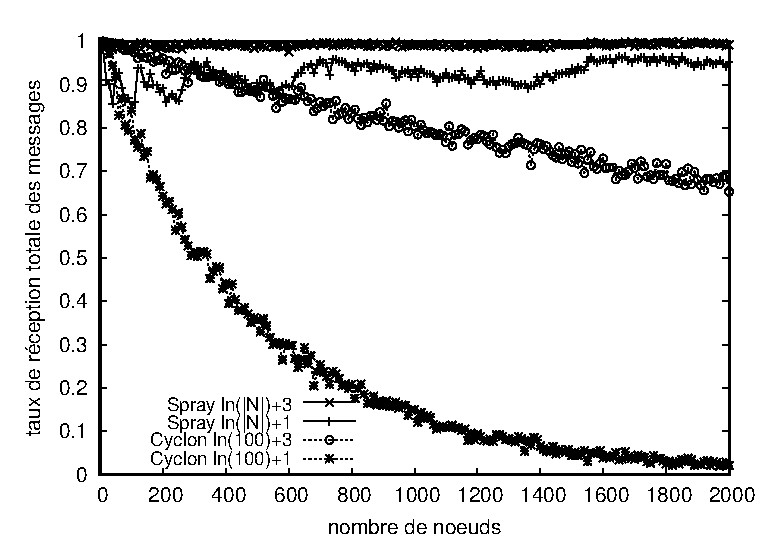
\includegraphics[width=1\textwidth]{img/network/hardrate.eps}
  \end{center} 
\end{frame}

\begin{frame}{Communication}{Le pic de popularité est mieux géré}
  \begin{center}
    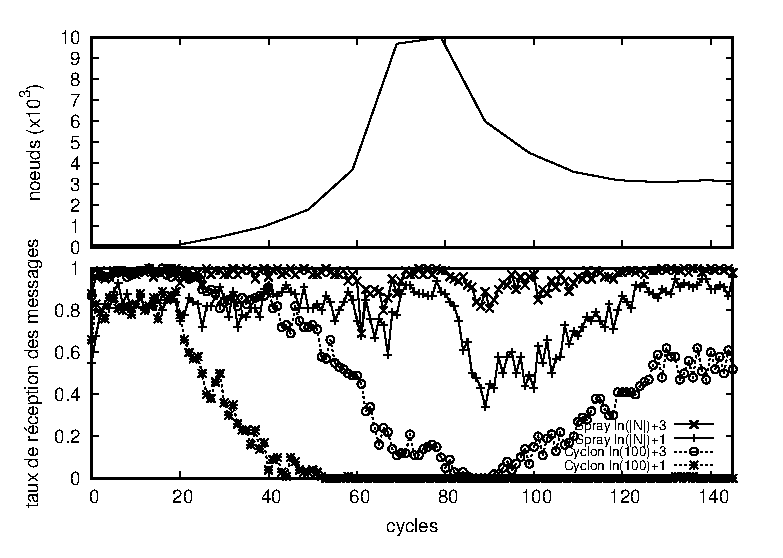
\includegraphics[width=1\textwidth]{img/network/peak.eps}
  \end{center} 
\end{frame}



\begin{frame}{Communication}{Conclusion}
  
  \begin{itemize}
  \item \SPRAY est un protocole d'échantillonnage aléatoire de pair adaptatif.
  \item \SPRAY est adapté au processus complexe d'établissement de connexion de
    WebRTC.
  \end{itemize}

  \vspace{0.25cm}

  \begin{itemize}
  \item \SPRAY a le désavantage d'utiliser des doublons, mais leur faible
    proportion n'impacte pas les propriétés du réseau.    
  \end{itemize}

  \vspace{0.25cm}

  \begin{itemize}
  \item Les protocoles construits au dessus de \SPRAY bénéficient de cette
    adaptativité.
  \end{itemize}

\end{frame}